%Background image credits:https://commons.wikimedia.org/wiki/File:CannabisBud.jpg Thomas Elliott, CC0, via Wikimedia Commons
\documentclass[a4paper, 11pt, oneside, polutonikogreek, english]{article}
\usepackage{lmodern}
\usepackage[T1]{fontenc}
% Load encoding definitions (after font package)
\usepackage[dvipsnames]{xcolor}
\usepackage{eso-pic,graphicx}
\usepackage[top=40mm, bottom=40mm, outer=34mm, inner=34mm]{geometry}
\setlength{\columnsep}{90pt}
\definecolor{customColor}{RGB}{221,229,194}
% Load encoding definitions (after font package)

\usepackage{textalpha}

\usepackage{listings}
\lstset{basicstyle=\ttfamily}
\usepackage{pdflscape}

% Babel package:
\usepackage[english]{babel}

% With XeTeX$\$LuaTeX, load fontspec after babel to use Unicode
% fonts for Latin script and LGR for Greek:
\ifdefined\luatexversion \usepackage{fontspec}\fi
\ifdefined\XeTeXrevision \usepackage{fontspec}\fi

% ``Lipsiakos" italic font `cbleipzig`:
\newcommand*{\lishape}{\fontencoding{LGR}\fontfamily{cmr}%
		       \fontshape{li}\selectfont}
\DeclareTextFontCommand{\textli}{\lishape}

\usepackage{booktabs}
\usepackage{graphicx}
\setlength{\emergencystretch}{15pt}
\graphicspath{ {./ } }
\usepackage[figurename=]{caption}
\usepackage{float}
\usepackage{fancyhdr}
\usepackage{microtype}

\usepackage{setspace}
\onehalfspacing

% change color of text, example replace all \color{Goldenrod} with \color{lightgray}

\makeatletter % change only the display of \thepage, but not \thepage itself:
\patchcmd{\ps@plain}{\thepage}{\bfseries\color{customColor}{\thepage}}{}{}
\makeatother

\color{customColor}

\begin{document}
\renewcommand\thefootnote{\bfseries\color{customColor}{\arabic{footnote}}}
\let\oldfootnote\footnote
    \renewcommand{\footnote}[1]{\oldfootnote{\bfseries\color{customColor}#1}}
\bfseries
\AddToShipoutPictureBG{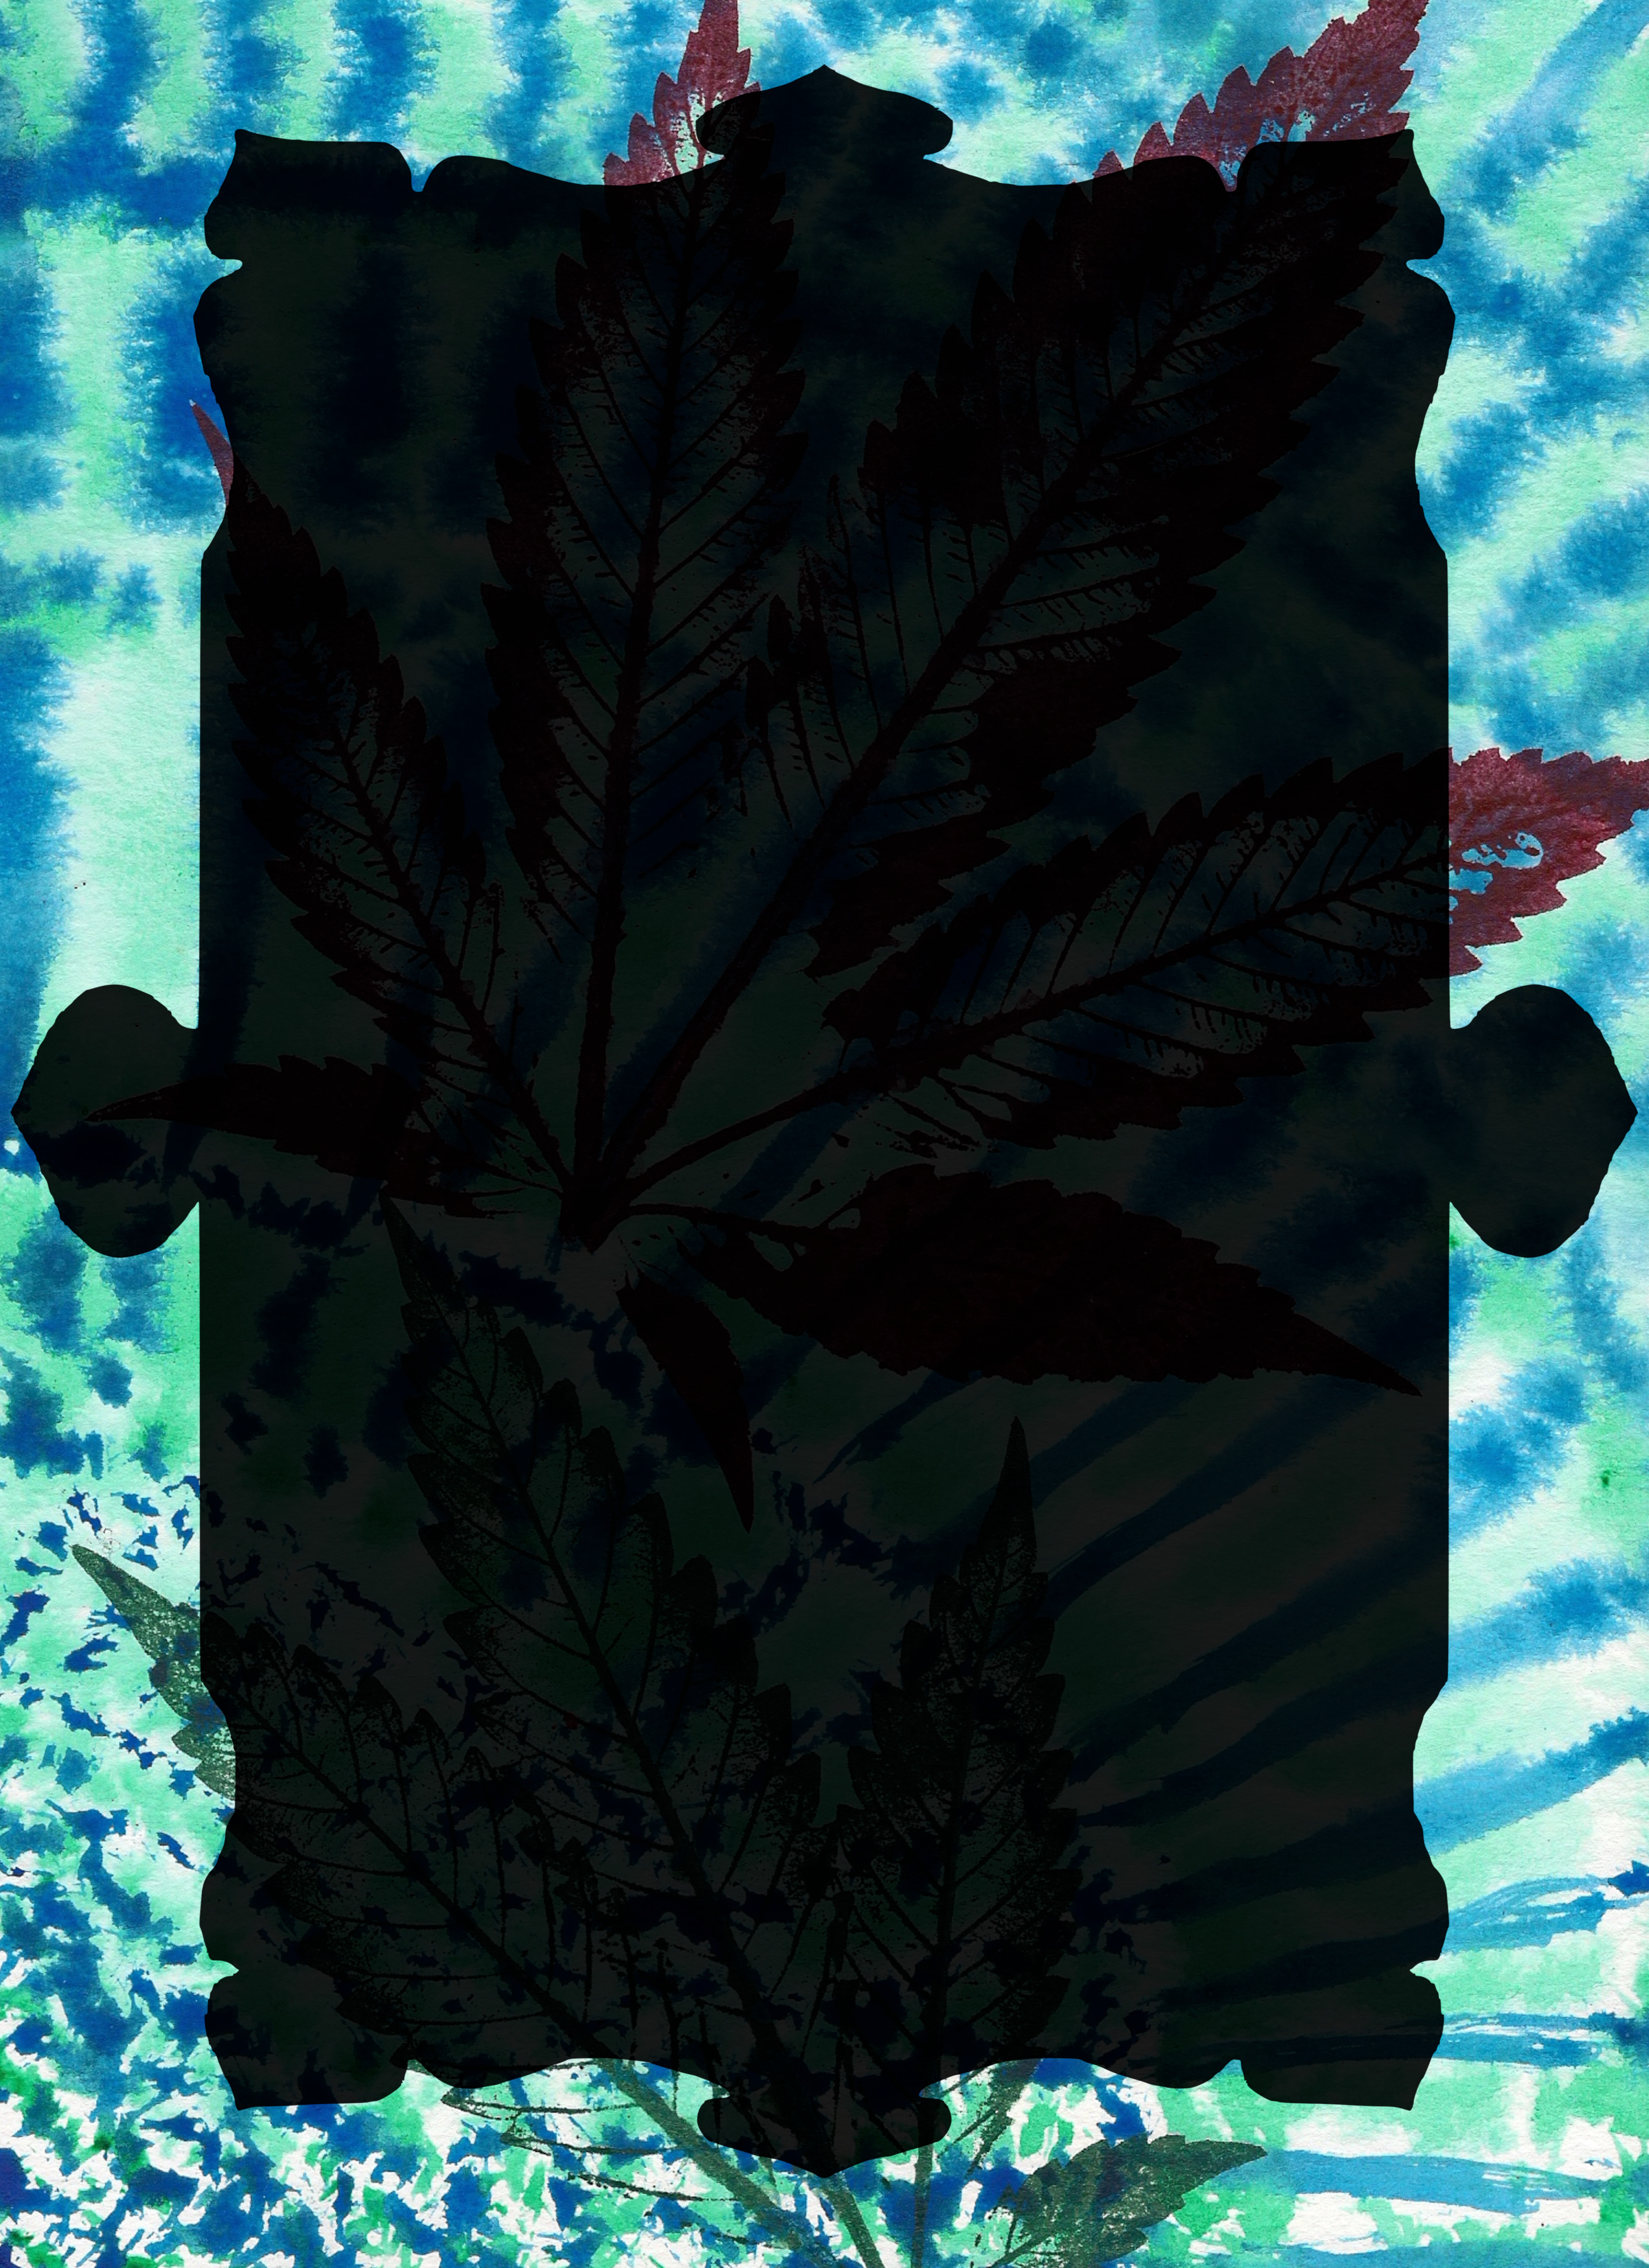
\includegraphics[width=\paperwidth,height=\paperheight]{hemp01.jpeg}}
\begin{titlepage} % Suppresses headers and footers on the title page
	\centering % Centre everything on the title page
	\scshape % Use small caps for all text on the title page

	%------------------------------------------------
	%	Title
	%------------------------------------------------
	
	\rule{\textwidth}{1.6pt}\vspace*{-\baselineskip}\vspace*{2pt} % Thick horizontal rule
	\rule{\textwidth}{0.4pt} % Thin horizontal rule
	
	\vspace{0.75\baselineskip} % Whitespace above the title

        {\LARGE A Treatise on Hemp \\} % Title
	
	\vspace{0.75\baselineskip} % Whitespace below the title
	
	\rule{\textwidth}{0.4pt}\vspace*{-\baselineskip}\vspace{3.2pt} % Thin horizontal rule
	\rule{\textwidth}{1.6pt} % Thick horizontal rule
	
	\vspace{1\baselineskip} % Whitespace after the title block
	
	%------------------------------------------------
	%	Subtitle
	%------------------------------------------------
	
	{Translated from the French of \\\Large M. Marcandier, \\\normalsize Magistrate of Bourges\\} % Subtitle or further description
	
	\vspace*{1\baselineskip} % Whitespace under the subtitle
	
	%------------------------------------------------
	%	Editor(s)
	%------------------------------------------------
	
	\vspace{1\baselineskip} % Whitespace before the editors

        {\small In Two Parts. Containing 1. Its History, with the Preparations and Uses made of it by the Ancients. 2. The Methods of cultivating, dressing, and manufacturing it, as improved by the Experience of modern Times.}

    %------------------------------------------------
	%	Cover photo
	%------------------------------------------------
	
	%\includegraphics[scale=1]{cover}
	
	%------------------------------------------------
	%	Publisher
	%------------------------------------------------
		
	\vspace*{\fill}% Whitespace under the publisher logo
	
	% Publication year
	
	{London, 1764} % Publisher
 
        {\small Printed for T. Becket, and P. A. de Hondt, in the Strand}

	\vspace{1\baselineskip} % Whitespace under the publisher logo

        Internet Archive Online Edition  % Publication year
	
	{\small Attribution NonCommercial ShareAlike 4.0 International } % Publisher
\end{titlepage}
\clearpage
\setlength{\parskip}{1mm plus1mm minus1mm}
\tableofcontents
\clearpage
\vspace*{\fill}
\begin{center}
To the Laudable Society for the Improvement of Arts, Manufactures, and Commerce, this Treatise on Hemp, as both curious and useful, is with the greatest Respect inscribed by their most humble Servant, The Editor.
\end{center}
\vspace*{\fill}
\clearpage
\subsection*{Advertisement.}
\paragraph{}
The Memoir on the preparations of Hemp, which M. Dodart, Intendant of Berry, published in 1755, for the use of that province,\footnote{Bourges, the capital of Berry, (a province celebrated for its Hemp) was one of the cities of Gaul mentioned by Pliny, where, in his time, so great a quantity of linen and Hempen cloth was made, that he even seems to reproach them with... \emph{Ita ne et Galliæ censentur hoc reditu? Montesque mari oppositos esse non est satis, et à latere Oceani obstare ipsum quod vocant inane Cadurci, Caleti, Ruteni, Bituriges, ultimique hominum existum uti morini, immo vero Galliæ universæ vela texunt.} Plin. l. 19. c. 1.} excited the curiosity of the public, with regard not only to the natural properties of that plant, but also to its origin and history.

Though this little work was intended solely for the instruction of manufacturers, some respectable persons, and particularly the Journalists of Trevoux, who were pleased to give a favourable account of it in the month of January, 1756, seemed to wish, that, on this occasion, we had collected all the interesting particulars, that History could furnish, of the use formerly made of Hemp, and the knowledge that the nations of remotest antiquity had of it. Others, more concerned about the improvement that may be made of it at this time, earnestly desired more circumstantial and particular accounts, not only with respect to the culture and methods of preparing this plant, but also with regard to the various uses that may be made of it, in several sorts of manufactures. Desirous to satisfy both, we have endeavoured to re-unite, in this Treatise, those researches and remarks, that seem to comprehend almost all that Hemp can present to the curiosity of the learned, and the utility of the manufacturer: But far from flattering ourselves that we have exhausted a subject so interesting, and so extensive, with regard to which a great many experiments still remain to be made, we hope, that the first effect of this essay will be, to excite men of greater ability to take under further consideration, everything that has relation to this valuable plant,\footnote{There is none that offers so great advantage to man; it even brings in more than corn. \emph{Nouv. Mais. Rust.} tom. 1. p. 680.} and its uses, which, perhaps, are as yet but very imperfectly known.

We shall give several extracts from different Authors, who have left us any notices of this plant, and its uses, either in Physick, or the Arts; we shall also give particular observations relating to economy, which is the principal design of this work, and add some remarks upon the bad practices, the frauds, the negligences, and abuses, that have creeped into this branch of commerce. In a word, we shall do everything in our power to attain the end of this work: What further remains must be expected from the government, and from the public.

\subsection*{To the Lovers of the Arts.}
\paragraph{}
The principal design of this Memoir being to carry to perfection those Arts, the knowledge and use of which are as extensive as they are necessary, we thought it no less proper to gain to our interest those who cultivate them, than those on whom they depend for protection. We therefore consecrate and dedicate this work to them; we submit our researches to the judgment of both; and if everything we advance has not the happiness to please all, we hope, that that part of this Essay which they are pleased to approve of, will, at least, obtain their indulgence for that, which they may think deserves not their approbation.
\clearpage
\section{Part 1. Containing its History, with the Preparations and Uses made of it by the Ancients.}
\paragraph{}
To pierce through the dark veil of remotest antiquity; to range, with our first parents, the fields and forests,\footnote{\emph{Cannabis in silvis primum nata est.} Plin. l. 20. When the origin of an art is unknown, we must be content with conjecture and hypothesis instead of true history; and we may be assured, that, in such cases, the romance is more instructive than the truth. Generally speaking, chance suggests the first essays; they are fruitless, and never heard of: Another takes up the affair, he meets with some little success, but so little that it makes no noise: A third begins where the second left off: A fourth proceeds in the paths of the third; and so on, till the last of all produces some excellent experiments; and only these last discoveries make a sensible impression. If we have this discovery from a stranger, national jealousy conceals the name of the inventor, and it remains unknown. The origin and progress of an art are not like those of a science; learned men communicate their thoughts to one another; they write, they make the most of their discoveries, they contradict, and are contradicted; these disputes are proofs of facts, and ascertain their dates. Artists, on the contrary, live in obscurity, and in a kind of solitude; they do all with a view to profit, and scarce anything for fame or glory. Some inventions continue whole ages, confined to one family: they are handed down from fathers to their children, and carried to perfection or suffered to decay; so that we know not precisely to what person, or to what time, we ought to ascribe their discovery. The insensible steps by which arts rise to perfection, contribute also to render their dates uncertain. \emph{One pulls the hemp, another waters it, a third peels it; it is at first a coarse twine, then a thread, and afterwards woven into cloth; but a whole age intervenes between every step of this progress.} Could one man carry a production from its natural state to the highest degree of improvement, it would be a very difficult matter to conceal his name. Should a people all at once find themselves clothed with a new kind of stuff, how could they avoid enquiring to whom they owed the discovery? But such cases never, or very rarely happen. \emph{Encycl. vol. 5. p.} 647.} and from all the plants, which cover the face of the earth, to select those which seem to have been, at all times, the most useful and necessary; in a word, to discover the origin of Hemp, and shew how mankind, from the beginning, have employed it, is an enterprise the more difficult, that historians throw no light at all on this subject, and we can by no means find to whom we owe the discovery thereof, nor of its uses.

It is to be presumed, that this plant having been cultivated, and applied to use, long before histories were written, the first writers did not think it necessary to speak of what was perfectly well known already, and at the same time very common.

I suppose, therefore, that chance or necessity, the two great springs of invention, at first discovered to men a plant as common as it is valuable. The first who made use of it wanted only, perhaps, a withe to tie up a branch, or a girdle for his waist. He found, in Hemp, flexibility, limberness, and strength. Upon this, he took particular notice of the plant, and observed its distinguishing marks. This was enough to make him communicate it to his family and his neighbours; everyone was sensible of the utility of this production for all sorts of ligatures. They would, no doubt, be disposed to multiply and render more common a plant, which appeared so very necessary: It was accordingly cultivated; but several ages, perhaps, elapsed, before anyone thought of separating the bark from the stem. It was, however, at last found out, that by this means its use might be rendered more considerable and more extensive. It will be easily believed, that the preparation of Hemp, by \emph{watering} it, was not at first performed so exactly as at present. They began, without doubt, with twisting it into small ropes,\footnote{\emph{Cannabis sativa planta, magni usus in vitâ, ad robustissimos funes factitandos.} Dioscor. l. 3. c. 141.  \emph{Utilissima funibus Cannabis.} Plin. l. 19. c. 9.} as the shepherds in the country still continue to do. Hereafter some set up rope-yards; others, probably, attempted to spin it, then made it into cloth\footnote{History informs us, that the weaver's looms, in ancient times, were of a frame very different from those we use at this day. The operators did not fit, but worked standing; and when they were employed on webs that were to be flowered on both sides, they turned round their looms.  \emph{Arguto tenues percurrens pectine Telas.} Æneid. 7.  Homer, Herodotus, Theophylact, \emph{etc.} acquaint us, that the warp of their hempen cloth was extended from top to bottom of the loom, and that, in applying the woof, which they struck home with a kind of wooden sword, they worked almost in the same manner with those that weave girths with us.}; but what sort of cloth must this have been? At last, as by degrees, arts, as well as men, are brought to perfection; after several thousands of years, Hemp came to be made into fine cloth; and none but persons of great experience could distinguish it from what was at that time made of Flax.

Herodotus, the most ancient historian, acquaints us, in the fourth book of his history, ``That, in his time, the people of Thrace cultivated a kind of Hemp, Κάνναβις, that very much resembled flax, excepting that the stalk of it rose higher. Some of it, says he, is cultivated, and another kind grows wild: Both these kinds are preferable to everything of the sort that we have in Greece. The Thracians\footnote{The Thracians, as we are told by Herodotus, \emph{l.} 5. were, next to the Indians, the most extensive of all nations: They derived their original and name from Teras, the son of Japheth, who was their Patriarch. In old times under this name were comprehended, not only the inhabitants of Thrace, but also the \emph{Getæ}, the \emph{Daci}, and the \emph{Mysians}: The names of \emph{Thrace} and \emph{Scythia} are also sometimes taken indifferently for one another.\\\hspace*{5mm}\emph{Nascitur autem apud cos (Scythas) Cannabis, Lino simillima, præter quam crassitudine et magnitudine, sed multo quan nostra præstantior, vel sua sponte nascens, vel sata, ex qua Thraces vestimenta conficiunt Lineis simillima; quæ nisi quis fit valde exercitatus, Linea sint, an Cannabea, non queat dignoscere, et qui non viderit Cannabem existimet Lineum esse vestimentum.} Herodot. Melp. pag. 281. edit. Græc. Lat. Henrici Stephani, ann. 1592.} make cloths of it, which are as beautiful to the eye, as those that are made of flax; and none can perceive the difference, but such as are perfectly acquainted with such manufactures.''

If it is plain, from this passage, that, a long time before the christian æra, Hemp was cultivated in Thrace, as well as in Greece,\footnote{The Hemp which was cultivated in Greece, was not so good as that of Thrace, but it made excellent ropes, as we shall see hereafter, and, without doubt, coarse cloth for sails, and other works of this sort.} and at that time made into fine cloth; may we not conjecture, that other neighbouring nations, with whom they had any correspondence, understood the use of it also. Can it be supposed, that the Chaldæans, the Babylonians, the Persians, and the Egyptians did not make use of it, at least for ropes,\footnote{\emph{Demisit ergo eos per funem de fenestra.} Joshua chap. 2. ver. 15. This rope is in the translation called σπαρτίον.} which is the first use to which it would naturally be applied? Is it to be presumed, that those famous buildings so much boasted of in antiquity, without excepting that stately tower, which was the first monument of the wickedness and industry of men, were carried to perfection without the help of ropes? Though the holy Scripture mentions only Flax, on all occasions relating to Hemp, or linen cloth, or garments made of these materials, and the Hebrew text has taken no notice of Hemp, under the name we give it, in imitation of the Greeks and Latins, this is no sufficient reason for believing that the Jews were altogether unacquainted with the use and properties of this plant. The term λίνον,\footnote{The term \emph{linum} and λίνον was used to express all sorts of materials proper for the construction of cloth and ropes, as we are told by Robert Stephens, in his dictionary of the Latin tongue; where he says, that λίνον is ἀπὸ τοῦ λινέω, \emph{antiquo Verbo, quod est teneo, quia Lino omnia tenentur}. On this subject he quotes several authors, who give this word nine or ten different significations.\\\hspace*{5mm}Linum pro Filo. \emph{Cels. l.} 7. c. 14.\\\hspace*{5mm}Pro Fune Nautico. \emph{Ovid.} 3. \emph{Fast.}\\\hspace*{5mm}Pro Verriculo. \emph{Virg.} 1. \emph{Georg.}\\\hspace*{5mm}Pro Vinculo. \emph{Id.} v. \emph{Ænæid.}\\\hspace*{5mm}Pro Velo Navis. \emph{Homer. Iliad.}\\\hspace*{5mm}Pro Linteo in quo dormitur. \emph{Id.}\\\hspace*{5mm}Pro Hamo Piscatorum. \emph{Id.}\\\hspace*{5mm}Pro Fidibus Nervorum. \emph{Id.}\\\hspace*{5mm}Pro Cassibus quibus feræ capiuntur. \emph{Ovid.} 3. \emph{Met.}\\\hspace*{5mm}Hence \emph{Lino Sparton}, not that sort of which sheets or sails were made, but a coarser sort of Flax, or Hemp, which was made into ropes.\\\hspace*{5mm}The word \emph{linteum}, for the same reason, was used to signify all those sorts of cloth, \emph{quæ ex cortice Lini, Cannabis, aut Byssi, texebantur}. We shall see hereafter, that the word \emph{Spartum} was of the same kind. \emph{Veteribus Græcis σπάρτον dicebatur, id omne ex quo fierent vitilia, aut funes, aliaque ad nexum idonea, ut sunt Linum, Cannabis, Junci, Genistæ, etc.} Vossius, Diction. Etymol.} or \emph{linum}, which is used by the Greek and Latin translators; ought to be considered as one of those general expressions that were much used in the Hebrew\footnote{The Hebrews, for instance, used the word \emph{Baal}, to signify all sorts of gods or goddesses.} and Chaldaic languages.

The Greeks, indeed, made use of a kind of broom, \emph{Spartum}, σπάρτον,\footnote{\emph{In Græcia Sparti copia modo cœpit esse ex Hispania, neque ea ipsa facultate usi Liburni, sed hi plerumque naves loris suebant. Græci magis Cannabo et stupâ, cæterisque Sativis rebus à quibus σπάρτα, Sparta appellabant.} Aul. Gel. l. 17. c. 3.\\\hspace*{5mm}\emph{In sicco præferunt è Cannabe funes.} Plin. l. 19. c. 2.\\\hspace*{5mm}This \emph{Spartum}, σπάρτον, has occasioned great difficulties among learned men. The Greek authors, and their Commentators, speak so differently of it, that it is still very doubtful in what sense it ought to be taken. Some pretend that its name is derived from \emph{satum}, id est, \emph{sativum}; while Pliny maintains that the \emph{spartum} of Spain \emph{sponte nasci, nec seri posse}. Others will have it to come from σπείρειν, \emph{nectere et complicare} (\emph{Hesychius, Suidas, Aristophanes, Pollux, vocant σπαρτία vel σπαρτίον funes vel funiculos quibus utebantur fabri ad varios usus, sive ex Lino, Cannabe, Junco, vel alia materia nexi fuerint, aut conserti.} Henr. Steph.), because the Greeks gave this name to everything that could bear to be spun and twisted: This is the opinion of the best authors. They use the word \emph{Spartum}, to express everything that is of the nature of Hemp, as the Hebrews did the word Flax to signify three sorts of things, which are often confounded in the Holy Scripture, \emph{viz. Bad, Linum}, the most common sort, which was used in the making of cordage and coarse cloth; \emph{Schesch, Gossipium}, a finer sort, sometimes taken for cotton, which was used in making clothes for persons of rank and distinction; \emph{Buz, Byssus}, very fine, which served for making ornaments for an use of the Priests and the Temple; it is scarce possible to imagine, that the Jews were entirely unacquainted with Hemp, which was so well known to other nations (\emph{Est enim verò Eleorum ager, et cætera ferax, et Byssum educat felicissime. Cannabem quidem Linum et Byssum serunt, qui idoneum ad hæc serenda solum colunt.} Pausan. lib. 6. ad finem.). It is much more natural to suppose, that it was one of these kinds of Flax we meet with in the several texts of Scripture, where mention is made of coarse, and fine linen, and of cordage. See Ezek. ch. 27. ver. 16; 1 Chron. ch. 6. ver. 21; ch. 15. ver. 27; and 2 Chron. ch. 2. ver. 14; ch. 3. ver. 14; Esth. ch. 1. ver. 6; ch. 8. ver. 15.} which they brought from Spain, for the service of their marine, and for caulking their ships, because it made greater resistance to the water than Hemp; but for ropes and every other purpose they preferred Hemp. Is it possible that Nineveh, Babylon, Memphis, Palmira, Thebes, and so many other famous cities should have been quite unacquainted with the use of a plant so necessary and so common?

The Romans made sails of it, and ropes for their sea\footnote{\emph{Tun' mare transilias tibi torta Cannabe fulto. Cœna sit transtro.} Pers. Sat. 5. ver. 146.} and land service. They had magazines of it in two of the principal cities of the western Empire; the Hemp necessary for the purposes of war, was, by the Emperor's | orders, amassed at Ravenna in Italy, and Vienna in Gaul. The officer, who superintended that matter on the further side of the Alps, was called the Procurator of the Hemp manufactures in Gaul, and had his residence at Vienna. Their husbandmen used Hemp for tying the oxen to the yokes\footnote{\emph{Cannabinisque funibus cornua jumentorum ligato.} Columel. lib. 16. cap. 2.}; and, without doubt, for all the other purposes relating to agriculture. We know that they made no great use of linen cloth, but they had some; and Vigenerus, upon Titus Livius, tells us, that they made use of Hemp: Even their laws and their annals were written on hempen cloth.\footnote{\emph{Licinius Macer auctor est et in fœdere Ardeatino, et in Linteis Libris ad Monetæ inventa... quæ si in ea re sit error, quod tam veteres Annales, quodque Magistratum Libri quos Linteos in æde repositos Monetæ, Macer Linius, citat identidem Auctores.} Tit. Liv. l. 4. c. 7. et 20.  It was in the temple of Moneta that the books of Hempen cloth, containing the destiny and fates of the Roman Empire, were kept with great care.  
The Samnites also made use of the same cloth for the purpose of writing. Tit. Liv. l. 10.} Nothing is more generally or better known than the use they made of it for adorning their theatres, covering their streets and their public places, their amphitheatres, and their \emph{arenæ} for the Gladiators, to shade those who assisted at their public shews. Plin. l. 19. c. 1.

Martial informs us, that the Romans also made use of hempen cloth for table linen, and that every guest generally brought his napkin with him.\footnote{\emph{Attulerat nemo mappam dum furta timentur.} Mart. l. 12.} We cannot therefore in the least doubt, but Hemp was known to the ancients,\footnote{We shall afterwards see to how many uses Hemp was formerly applied.} as a material of cloth for the service of war, both by sea and land,\footnote{\emph{Ubi vis magna Sparti fuit ad rem nauticam congesta ab Asdrubale.} Tit. Liv.} as well as for the purposes of agriculture. And if the greatest part of authors have sometimes made use of the word \emph{Spartum},\footnote{\emph{Sparteus generaliter pro quovis funiculo ponitur, sive è Sparto nexus fit, sive è Cannabe, Lino vel aliunde.} Athen. l. 5.} to signify ropes; even when those ropes were made of Hemp, the reason was, because they considered \emph{Spartum} as a general term applicable to Hemp as well Flax, or any material of that kind\footnote{\emph{Græci Juncos quippe ipsos, et Genistas, et quidquid denique ad funes nectendos, et aliquid ligandum verti posset, σπάρτον vocavére: hi autem vocem hanc σπάρτον, de herbis omnibus ad vitilia, nexilia, textiliaque aptis usurparunt...} Salmas. Exercit. Plin. pag. 261... and he adds: \emph{...ex Lino Hispanico, quis putet rudentes navium tortos unquam fuisse? Nugatur itaque Solinus, nec enim ad id dixit Mela. Ex Lino tamen armamenta navium etiam olim fuisse, eruditioribus placuisse, ibidem notat Plinius, qui versum Homori ita interpretabantur, quoniam cum sparta dixit significaverit sata. Quæ non intelligo, quasi necesse sit σπάρτον, nomine Linum accipi, quia significaverit sata. An non et Cannabis sativa, de qua τὰ σπάρτα, id est sata, in illo Homeri loco possumus interpretari... Nugatur itaque Solinus, nisi dicamus eum sub materie rudentum, Spartum tantum comprehendisse.}  The \emph{Spartum} of Spain, which we interpret \emph{broom}, is a sort of rush, \emph{Juncum aridi foli}, that grows near Carthagena; it is prepared almost in the same manner with Hemp by \emph{watering}; it naturally grows in that soil, and cannot be raised from seed.  
The Greeks also made use of another kind of rush for making ropes, which from thence had the name of χοῖνος.}; unless the signification of it be otherwise absolutely determined. In a word, how much should we know of the use that was formerly made of Hemp in China and Japan, and so in both hemispheres, if their histories had come with more accuracy into our hands.

We read in Kolben, that the Hottentots use a plant, named \emph{Dakka}, instead of tobacco, or at least mix them together, when their provision of the latter is almost exhausted. This herb, says he, is a kind of wild Hemp, which the Europeans sow principally for the use of the Hottentots.\footnote{\emph{Histoire Generale des Voyages}, l. 15. \emph{Hist. Nat. du Cap. tirée de Kolben}.}

Though the etymology of the word Hemp does not appear to be a matter of great importance, we think it our duty not to omit it, that we may leave nothing untouched that can be proposed with regard to this plant. Some pretend that it comes from the Celtic word \emph{Canab}\footnote{Pezron. \emph{Cannabis, Græcè Κάνναβις, vel Κάνναβος, unde et Belgicum} Kennep, \emph{quasi} Kannab, \emph{herba est funibus faciendis idonea, à Lino, et tenuitate, et candore distans. Est verò Κάνναβις, Κάννα.}}; others think they find its root in the Greek word Κάννα, or Κάννη,\footnote{Vossius.} which comes from the Hebrew \emph{Kannab}; in Latin \emph{Canna}; in French \emph{Canne}; because its form, and the length and size of its stalk give occasion to compare it to a cane. And therefore, as we say, a sugar-cane, \emph{etc.} we may also say, a hemp-cane. The terminations of particular languages, such as Κάνναβις or Κάνναβος, in Greek; \emph{Cannabis} or \emph{Cannabum} in Latin; \emph{Canapo} in Italian; \emph{Canamo} in Spanish, \emph{etc.} are so many expressions peculiar to those languages, but that variety makes no alteration in the signification.

Hemp is commonly distinguished into two sorts; one that grows wild, \emph{Cannabis silvestris}; the other produced by cultivation, \emph{Cannabis domestica}. This latter is of two sexes; the male \emph{fructifera}, and the female \emph{florifera}; but both improperly so called, for it is more natural to call that the \emph{female}, which bears the fruit, than the other that bears the flower. The seed and the root of wild Hemp, are like those of the wild mallow; the stalks are smaller, blacker, more rough, and about a foot and half in height; the leaves are like those of Hemp raised by cultivation, but more rough, and likewise blacker.\footnote{\emph{Nigriore folio et asperior.} Plin. l. 20. c. 23.}

The root of Hemp produced by cultivation is six inches long, or thereabout, of a whitish colour, ligneous, undivided, and running to a point, having fibres only on two lines, diametrically opposite to one another, when it is not straitened for want of room; and thick in proportion to the stalk it bears. The stalk is round, from the root to the first ramification; it then assumes a quadrangular form, and is fluted, hollow, ligneous, covered with a greenish bark, composed of filaments, hairy and rough to the touch: at proper distances this bark is secured from place to place by six small fastenings, which keep it close to the stem, like so many little nails, regularly ranged on the circumference of the same circle, and almost equally distant from one another. Its length and thickness are various, according to the difference of the soil, of the method of cultivation, of the climate, and of the seasons. Some of it rises to the height of eight or ten feet, and the stalks look like so many little trees\footnote{\emph{Quod ad proceritatem attinet, Rosea agri Sabini arborum altitudinem æquat.} Plin. l. 29. c. 9.}; others seem to pine away on the ground, and scarce get to the height of two or three feet, sometimes less. A grain of Hemp-seed, sown by itself, in a soil that agrees with it, commonly produces a stalk very large\footnote{Of such stalks they make a kind of charcoal, fit to enter into the composition of gunpowder.} and firm, with many branches, and looks like a little tree. If it is of that sex which produces seed, it will yield a great many grains, and those very beautiful: But its bark being too hard and thick, will not be very fit for manufacturing: On the contrary, seed sown in a field, that is properly prepared for the purpose, and near to each other, produce stalks that are straight, smooth, without branches, softer,\footnote{\emph{Quo densior eo tenuior.} Plin. l. 19. c. 9.} and more tender than the former; and the bark of such being smooth, fine, and soft, is much valued for several uses. The leaves grow two and two opposite to one another; they are divided into many segments, being narrow, oblong, sharp pointed, jagged, full of veins, of a deep green colour, rough to the touch, and of a strong smell, that affects the head.

The flowers that grow on the female stalk, as it is commonly called, issue from the \emph{alæ} of the leaves, on a pedicle of four little clusters, lying in the form of a Saint Andrew's cross: They have no \emph{petals}, and consist of five stamina, with yellowish summits, in a calyx of five leaves, of a purple colour without, and whitish on the inside; these flowers are not followed by any fruit; and, on the other hand, the fruit on the stalks that produce it, is never preceded by any flower.

Whatever the order of nature may be in the vegetation of this plant, both the male and the female stalks are produced indiscriminately from the grains of seed that grow on the same stalk; and the difference cannot be known till they come to blossom. We know not, when we sow Hemp, what quantity of either sex will be produced, nor which contributes most to the propagation of the plant; they cannot, however, be easily distinguished till\footnote{The time when the Hemp blossoms cannot be exactly ascertained; for it depends on several circumstances. Sometimes it is not above a foot high; when this is the case, the Hemp continues weak, and grows little or nothing at all higher; this is sometimes occasioned by great heats, or other unfavourable accidents; at other times it rises to the height of four or five feet before it blossoms, and grows almost as much after. The Hemp, which bears the flower, commonly gets before that which produces the seed, and rises about half a foot above that which bears the grain. This superiority, in the order of nature, may be well accounted for, if it is true, that the powder, which issues from the flower, serves to convey fertility to the grain on the stalks that bear the seed.} sixty days after they are sown; but this observation, hitherto, does not appear to have been of any consequence.

The fruit grows in a great number of bunches at the end of the stalks and branches, which naturally produce them: This fruit is terminated by a forked style, when it is in \emph{embryo}, and is wrapt in a membrane, which secures it till it comes to maturity; then the pistillum changing to a roundish grain, forces the membranous capsulæ, which contain it, to open, and we therein discover a round smooth grain, somewhat flattened, and of a shining grey colour, containing, under a thin shell, a tender, sweet, and oily, white kernel, of a strong smell, that intoxicates when it is fresh. This kernel is covered with a green pellicle, terminating in a point on the side next the germ, which is very singularly situated.

This grain, which is called \emph{Hemp-seed}, is no less useful for its peculiar qualities, than for those which it has in common with the whole plant. Its substance, considered as a seed, is soft, fat, oily, and gummy; it ferments, conceives heat, and springs up with equal facility; its pores being large, tender, and flexible, receive greedily the impressions of heat and humidity, which transmit to them the nutritious juices supplied by a fat, light, and well-laboured soil; its fibres, after a quick germination, unfold themselves, grow up, and attain strength, and the gum, being the principle of their union, supports and preserves them. Besides the use of its oil in Physick, it is also employed, with great advantage, in the lamp, and in coarse painting: They give a paste made of it to hogs and horses, to fatten them; it enters into the composition of black soap, the use of which is very common in the manufactures of stuffs and felts; and it is also used for tanning nets.

A grain of Hemp-seed, seen by the help of a microscope, presents at first a greyish epidermis, full of veins, the compartments whereof appear like a sort of scales. Under this first cover you see a brown olive coloured bark, extremely smooth on the inside, formed of two shells, which separate exactly in the middle, like those of a nut, the seam that joins them being quite imperceptible. Under a green cover, its kernel, in the form of a little orange, bears its germ produced along one of its sides, which makes it look a little flatted: When you have taken up this pellicle, you find a white kind of matter, consisting of two lobes joined together, which evidently form a kind of head; these lobes are very distinct, and by the germination are made to swell, open, and separate. Its germ, which is roundish, bending back along the whole external length of the grain, under the seam which joins the two shells, terminates in a point, and forms a kind of tendril, which is the only part that pierces the ground to form the root; the other end of the germ, which lies concealed between the two lobes that enclose and preserve it, appears like an exceeding fine and delicate sort of lance\footnote{Which they call \emph{the feather}.}; from it issue the two leaves that appear first, and we may imagine it to be the true principle of its germination and life. These two lobes are also changed into two sorts of thick green leaves,\footnote{Which the Botanists call \emph{the seminal leaves}.} of an oval form, but not indented, which serve for a rampart, and preservative to the springing leaves. The whole of this white matter seems to be fat and spongious; and its pores appear to be no less open than those of snow: And it is, no doubt, owing to the situation of its germ, and the softness of its whole substance, that Hemp-seed, beyond any other sort of grain, has so great a disposition to ferment, and spring up almost as soon as it is sown.

The bark, as it appears upon the stalk, forms a green, knotty, rough or prickly covering to it. These knots and prickles are mere excrescences of gum, of which the whole bark is composed; but they have different degrees of force and adhesion. This first superficial gum serves only to keep the fibres of the Hemp close together, and as a kind of mastic to cover, strengthen, and protect them, against the inclemency of the air, the dust, and the rain: It dissolves, exfoliates, and breaks, when the bark is watered.

The inside of the bark, which touches the stem, is smooth, soft, and white; the fibres are very distinct from one another, and appear perfectly in all their dimensions, by means of the watering just mentioned. It was not observed in former times, that the thread had its existence in the plant, without any dependence on the operations of art; that the labour is confined to cleaning, dividing, and separating the soft fibres of which the bark is composed; and that this bark is a kind of natural ribbon, or scarf, the threads whereof are applied and joined together, lengthways, only, by a dirty glutinous humour, which must absolutely be dissolved and separated, because it is equally hurtful to the workmen and the work. The threads themselves also consist merely of a gum, but of one that is of a different quality from the superficial gum; they are supple, strong, and resist the impressions to which the former give way. Every fibre is composed of gummy globules, that are very fine, transparent, and bright, when sufficiently cleared from that superficial gum that surrounds them; and which the microscope shews to be of a different sort. All this will appear plain, if you take a few fibres from a thread that is thoroughly bleached. The fibres of Hemp, in this state, are nothing different from those of cotton and silk, which makes it reasonable to consider them as materials of the same kind: And it is a convincing proof of this, that when they are mixed and carded together, there appears to be a complete sameness in the whole mixture.

We should have found, without doubt, more curious and circumstantial observations, in the generality of authors who have examined this plant, if they had been as fully persuaded of its utility in the arts, as of its medical properties.

Pliny tells us, that Hemp-seed is of a drying nature, that it weakens the generative powers in men,\footnote{\emph{Semen ejus extinguere genituram virorum dicitur...} l. 20. c. 23.} when they eat it to excess. On the contrary, it promotes fruitfulness in fowls, for which reason it is purposely given them in wintertime, and is a food to which birds are accustomed. It expels wind; is hard of digestion; and disagrees with the stomach; it produces bad humours, and occasions headachs.\footnote{\emph{Sed cum dolore capitis.} Ibid.} It was formerly one of those legumes, which were fried for deserts.\footnote{De la Mare, \emph{Traité de Police}.} It was also made into little sweet cakes, to be eaten at collations, and to promote drinking; but, at present, this unwholesome ragout is quite banished from our tables: It heats those that eat it too freely so much, that it occasions very dangerous vapours\footnote{Gallien, lib. 7. \emph{de Simpl. Medic.}}; so that those who prescribe a decoction of this seed to children that labour under epilepsies, far from procuring them relief, increase and irritate their disorder. The juice of it,\footnote{\emph{Succus ex eo vermiculos aurium, et quodcumque intraverit, ejicit.} Plin. l. 20. c. 23.} squeezed out when it is green, draws insects to it, and brings out all the vermin that enter into the ears, and infest them. Taken in an emulsion,\footnote{We meet with this in several authors who boast of its effects. See \emph{Emulsio Cannabina ad Gonorrhœam}, de Doleus, Etmuller, Michaëlis, et Minschit, \emph{etc.}} it is good against a cough and the jaundice, and also against the gonorrhœa; its oil is recommended as an ingredient in pomatums for the small-pox; and it is laxative. Taken inwardly, or outwardly applied, it has not the dangerous qualities that are ascribed to the whole plant with its leaves; the powder of it, mixt with drink, will make those who use it drunk, dull, and stupid: We are told that the Arabians\footnote{De la Mare, \emph{Trait. de Pol.} l. 5. tit. 15. Where he quotes Simeon Sethi, \emph{De aliment. facul. C. Apitii, de re culinar.}} make a sort of wine of it, which intoxicates, and poor people eat the oil of it in their soup.

The grain and the leaves being squeezed, while they are green, and applied, by way of cataplasm, to painful tumours, are reckoned to have a great power of relaxing and stupefying. The smell of it is extremely strong and intoxicating. It is pretended, that the water, in which Hemp hath been steeped, proves a deadly poison to any that drink of it: This may be true; but what is commonly said of the same danger to fishes in the rivers\footnote{The Ordonance of Waters and Forests on this subject seems not to be well founded.} and ponds, in which Hemp is watered, is false. Fishes love this plant, and fly to it; but if any accidents of this kind should happen, they can only be owing to the smallness of some reservoirs, where the water not having a free course, may be too much impregnated with the juice of the Hemp, or afford to the fish too much of a delicious food, an excess of which is aways hurtful.

What Pliny assures us, of the great effect which an infusion of Hemp may have in coagulating water,\footnote{\emph{Tantaque vis ei est, ut aquæ infusæ eam coagulare dicatur, et ideo Jumentorum alvo succurrit pota in aquam.} Plin, l. 20. c. 23.} will not appear surprizing if we attend to the quality and quantity of the gum, which unites all the fibres of this plant together, and whereof, in reality, it entirely consists. It is, doubtless, for this reason, that it is given in drink to cattle to cure looseness. The decoction of green Hemp, with its seed, when well cleared of the dregs, causes the worms to come out of the ground on which it is poured, and the fishermen commonly make use of this expedient to catch them, when they have occasion.

Matthiolus presumes, that it may also have power to drive worms out of the human body. It is given in a drink to cattle and horses troubled with a looseness; the whole substance of the Hemp being gummy, it is by no means surprizing that it should have a restringent quality; and this is the reason why the powder of its leaves, taken in drink, is reckoned good for dysenteries, and the dust of the Hemp itself, which the labourers draw in with their breath, when they are at work upon it, causes obstructions in their lungs, and almost always, makes them asthmatic.

The root of it\footnote{\emph{Radix contractos articulos emollit, in aqua cocta; item podagros et similes impetus: Ambustis cruda illinitur, sed sæpius mutatur priusquam arescat.} Plin. l. 20. c. 23.} boiled in water, and applied in the form of a cataplasm, softens and restores the joints of fingers or toes that are dried and shrunk. It is very good against the gout, and other humours that fall upon the nervous, muscular, and tendinous parts. It abates inflammations, dissolves tumours and hard swellings upon the joints. Beat and pounded in a mortar, with butter, when it is still fresh, it is applied to burns, which it relieves greatly when it is often renewed. The juice and decoction of it, put into the fundaments of horses, brings out the vermin that infest them.

Even the lint\footnote{\emph{Repertaque linteorum lanugo, è villis navium maritimarum maximè in magno usu medicinæ est, et cinis spodii vim habet}. Plin. l. 19. c. 1.} which is yielded by hempen cloth, especially that which comes from the sails of vessels, is very much esteemed in physic, and the ashes of these sails serve for Spodium, Lapis Calaminaris, or Tutty.
\begin{center}
End of Part 1.
\end{center}
\clearpage
\section{Part 2. Of the Methods of cultivating, dressing, and manufacturing it, as improved by the Experience of modern Times.}
\paragraph{}
After having laid before the reader, in the former Part, all that our researches could produce with respect to the Natural History of Hemp, the object that appears to us most interesting, is its Cultivation.

The ground intended for the Hemp-field, ought to be the very best that can be afforded, either near the house,\footnote{\emph{At pauper rigui custos alabandicus horti}\\\hspace*{5mm}\emph{Cannabias nutrit silvas, quam commoda nostro}\\\hspace*{5mm}\emph{Armamenta operi! gravis est tutela, sed ipsis}\\\hspace*{5mm}\emph{Tu licet Æmonios includas retibus ursos.}\\\hspace*{5mm}Gratian. in Cyneget. v. 46.} or along some stream, or water-ditch, yet so, that there is no ground to fear an inundation. To render this ground fruitful, we must not spare either manure or labour. Hemp-grounds must be dunged every year, and the better to secure success, it would be proper to lay on the dung before the winter tillage, that it may waste itself there, and mix the more perfectly with the ground, which, impregnated with these new salts, will derive the greater advantages from the influences of that season, and catch more of the volatile salts of the air, that commonly abound most in the winter.

Of all the sorts of dung, that are used for Hemp-grounds, pigeons-dung only, or any other kind of dung that is fully ripe, ought to be laid on before the last labour; as is practised with success in several places. In countries where the land is strong they generally lay it in heaps after Autumn. In this manner it becomes more free and light, than when it is only tilled. The snow and rains, which penetrate it in the winter time, and the frosts that are common in that season, kill, if we may so express it, that ground, as they would a chalk-stone, and make it so free, that in the month of February nothing more is wanting, but to lay it level by a quick and easy labour. All its parts, and even the most tender particles, will be then found extremely small, light, and lively.

But different soils require different methods of preparation; and it is the part of men of understanding to discontinue bad customs, that have prevailed till this time, and substitute better methods in their place.

Hemp is one of those plants, which Nature has hot only made necessary, but also common, and suited to every sort of soil, as well as to every climate. It is true, that countries which are extremely hot, are not favourable to it; but as this plant is but a short time in the ground, if a country is at all habitable by men, we are of opinion they may also cultivate Hemp. Rainy seasons are proper enough for sowing it, and when it is once in condition to cover the ground, the dews alone, which are plentiful in these countries, will be sufficient to bring it to maturity. It will not, to be sure, grow so high as in temperate, or colder climates, but it may be, perhaps, on that very account, the more fit for use.

We find, by experience, that in temperate climates, \emph{France for instance}, the Hemp cultivated in the southern provinces has better qualities than that which grows in the northern, where the ground is fat, and not so warm.

In the north of America and Europe, Hemp thrives exceedingly well: that commodity is exported from thence into England, Holland, and even France, to the shame and detriment of those that cultivate it with us. Could no means be fallen upon to encourage them, and increase their number? What country is in better condition to apply to it, and profit by it, than France?\footnote{The Council passed some Acts in December 1719, and in May and June 1722, which it would be proper to consider.} All her provinces produce very good Hemp; and, instead of taking it from strangers, we ought to put ourselves in condition to sell it to them. Guyenne, Languedoc, Provence, Dauphiny, Auvergne, Burgundy, and Berry produce as good Hemp as can be wished, and nothing is wanting but the best methods of cultivating and preparing it.

The first, and most important operation, ought to be performed before winter. Some do it with the plough, others with the pick-axe, and others with the spade; the last of these, without doubt, is the best, because it goes deepest and makes the ground more free.\footnote{\emph{Deinde utilissima funibus Cannabis feritur à favonio} Plin. l. 19. c. 9.} In the beginning of the spring the ground is prepared by fresh labour, for receiving the seed, in such manner, that not so much as one clod be left unbroken, and the whole field be as smooth and in as good plight as a plot in a garden.

To have good seed you must use the produce of the last crop, and the grain must be clean and full grown. Seed of two years growth will not be so good, that of three years standing will be still less valuable; and oftentimes will not spring up at all. You must neither sow too thin, nor too thick\footnote{General rules cannot be given on this head; much depends on the ground and on the seed; it is certain, however, that it is sown thicker than corn.}; both excesses have inconveniences that inseparably attend them. Yet the danger of sowing too thick is the greater. For, besides the loss of the seed, that might have been saved, the ground being drained of a great part of its juices, while the seed is springing up and getting out of the earth, will not have enough left to bring it to perfection; by this means a great many stalks, especially those that are latest in springing, are quite choaked\footnote{\emph{Quo densior eo tenuior.} Plin. loco cit.}; or if this should not be the case, yet still they languish for want of nourishment, and the Hemp produced has neither the length nor strength it would have acquired, had it been sown thinner.

The season for sowing it begins not much before the first of April,\footnote{\emph{Hoc tempore Cannabum seris.} Palladius, l. 3. c. 6.} and does not last beyond the end of June. The diversity of soils in the same province, and the inconstancy of seasons, occasion this difference. And so long a season for sowing is the more necessary, that it gives an opportunity to sow the same field a second or third time, when, by reason of various accidents, the first seed is lost. But after all, the Hemp that is first sown generally thrives best, and appears most beautiful, unless it is nipt by the frost, or spoiled by the heat, when it begins to spring and grow up. The day on which this plant springs, and a few that follow it, are generally most critical; but, in a short time, it acquires strength enough to bear all the cross accidents that can befall it: A little rain before or after the Hemp is sown, turns much to its advantage.

When the seed is sown, it must be put under ground, either by means of the harrow, if the field has been tilled with a plow, or with the rake, if it has been done by hand; but, however well the seed may be covered, you must not lose sight of your field till the Hemp gets fairly above ground. The birds, especially the pigeons, are enemies, which must be continually kept at a distance. Though they do not scratch, nor do the least injury, to corn newly sown, when the seed is well covered, yet they are still dreadful to Hemp-seed, which rises quite out of the ground when it springs; whereas all other sorts of grain lie concealed in it; and therefore the pigeons, perceiving the Hemp-seed at a distance when it rises and discovers itself, pick it up, and all is lost. This is almost the only attention which Hemp-grounds require, from the seed-time to the harvest. Those which are situated on the sides of streams or rivers, or surrounded by ditches, may be watered in time of great drought. In countries where their situation will allow it, they are drenched by letting the water run in upon them. This labour and attention in the person who cultivates Hemp, often turns out to his advantage, and is well rewarded. When the ground is sown too thin, or by any accident the grass gets up and injures the Hemp, the superfluous stalks, or weeds, must be carefully pulled up, for fear they should be prejudicial to the rest.

Towards the end of July, the stalks which bear the flower, and are improperly denominated \emph{female}, begin to grow yellow at the top, and white at the root, the flowers fall, the leaves wither, and this is generally the sign of their maturity. They are then pulled up,\footnote{There would be danger in letting them stand longer; for besides that they would hurt the rest, they would themselves become useless, and by drying in that position would lose their strength and their other good qualities.} and made up in small bundles, which are ranged upon the verge of the field, taking care, as much as possible, to place the stalks, which are of the same length, equal at both ends, but especially at the roots. It must also be observed, in pulling up these stalks, not to hurt those that are to stand and bear the seed. This done with proper caution, will give new strength to the plant that is left in the ground. For this kind of weeding not only delivers the Hemp-ground from a great number of plants, that exhausted its strength, and injured and choaked one another, but is also an operation useful to the rest that remain, by raising and stirring the ground about them.

In some places, after binding the small bundles with the worst stalks of Hemp, they expose them to the sun, to dry the leaves before the Hemp be watered\footnote{The word \emph{Rouir}, which we translate \emph{to water}, is by some derived from \emph{Ros, Dew}, because in some places Hemp is exposed to the dew, to be watered thereby. In low latinity, it was ordinary to say \emph{Rohiare} for \emph{Rouir}, and \emph{Rothorium} to signify the place where the Hemp is watered. \emph{Ducange.}  In the Ordonance of the Emperor Frederic, which makes the thirty-fifth title of the third book of the Constitutions of Sicily, this operation is called \emph{Cannabum maturare, macerare, diluere, aqua subigere}.  Others pretend that the word \emph{Rouir} is derived from the red colour which the Hemp contracts during this operation.}; and when they are dry enough, they cause them to fall off, by striking every bundle against the wall, or a tree, or the ground: But this does not appear to be the best method; because, besides that it multiplies toil and labour, it also exposes the Hemp to many accidents, when the season happens to be rainy. The water which falls upon the Hemp before it is dry, makes it of a blackish colour, and full of spots. This inconvenience might be avoided, by observing a method, which to us appears to deserve the preference. When the Hemp is perfectly ripe, for this is a circumstance absolutely necessary, it must be put into the water as soon as it is pulled out of the ground. It's gum, which then is, in some respect, in a state of fusion, will consequently be the more quickly dissolved.\footnote{For greater accuracy, it would be proper to cut off both the extremities of the stalks, but especially the roots, which serve only to spoil the rest of the Hemp.} In this condition it will not require to be more than four days in the water: whereas when it is not watered till after it is dry, it is a matter of much greater difficulty to dissolve it, and it must lie in the water eight or ten days, and sometimes more, according to the seasons. Warm water forwards the effect of watering, and cold retards it.

All that are employed in the cultivation of Hemp, know how it is commonly laid down, in order to be watered. It is covered with a little straw, to keep the dirt from sticking to it, and loaded with pieces of wood and large stones, or other heavy materials, that it may be always five or six inches below the surface of the water.

As the physical effect of watering\footnote{Many have believed that the operation of the watering was the beginning of putrefaction over all the parts of the plant, without distinction, and was necessary in order to break the stems with greater ease: but this is without foundation: the stem would break as well if it was not watered at all; but the Hemp could not so easily be separated from it, for the reasons that we assign. In a word, should the Hemp lie in the water some days more or less, the difference would not appear on the stem, but it would be very sensible, and of very great consequence in the bark.} was not formerly enquired into, they fell into some mistakes, the consequences of which were not perceived. The watering of Hemp producing only a proportional dissolution of a certain quantity of the gum, which joins all the fibres of the Hemp together, and attaches them to the stems; it is of some consequence to observe where, when, and how this dissolution is effected. The finest and clearest water is always the best. Some make a kind of ditch on the edge of a river, where the water, being more still and warm, ferments easily, and penetrates more quickly the parcels of Hemp that are laid in it. When they are taken out of this ditch, it will be sufficient to wash them in the current of the river, which will carry off all the gum and mud that would otherwise cleave to them. The Hemp that is watered in rivers is always the whitest, and of the best quality. That which we are obliged to lay in ditches, pools, or reservoirs of standing water, and unfit for the purpose, is always of a bad colour and a very disagreeable smell, loaded with dirt, and loses a vast deal in the dressing.

In whatever manner this operation is performed, we know that the Hemp is sufficiently watered, when the bark is easily separated from the stem. This we find out, by drawing out, every day, a few stalks for trial. It would be dangerous to let the Hemp lie too long in the water; the fibres of the bark, too much divided, by an undue dissolution of the gum, would not have strength enough to stand the effort they must sustain, when the Hemp is peeled or braked, and a great part of it would remain with the stems, and be lost in the braking.

It is therefore necessary, for this very reason, to leave the Hemp no longer in the water than is sufficient to separate the bark from the stem, accurately and without loss. The same precaution must be used with the Hemp that bears the fruit, and remains, for ordinary, five or six weeks on the ground, after the other is pulled, that it may come to perfect maturity. This delay is far from being of any prejudice to the plant, as some have imagined; the bark, as it ripens, acquires all that force and resistance, which is suitable to its nature, and becomes preferable, especially for the construction of ropes, which cannot be too strong or too solid.

In the beginning of September,\footnote{\emph{Semen ejus cum est maturum ab æquinoxio autumni defringitur, et sole, aut vento, aut fumo siccatur.} Plin. l. 19. c. 9.} or rather, when the seed appears to be well formed, ripe, and ready to fall of its own accord, the Hemp is to be pulled as before, and in the same manner ranged in parcels. In some places, to bring the Hemp-seed to perfect maturity, and dispose it to leave the husks with greater ease, they make in the Hemp-ground, at proper distances from one another, round pits, one foot in depth, and six in circumference. In these pits they range the parcels of Hemp, quite close to one another, with the tops down, and the roots aloft. In this position, they confine them with straw ropes; then round this large sheaf they place the ground, that was taken out of the pit, that the tops may be effectually covered. The heat of the ground, and the humidity of the leaves, bring on a kind of fermentation, which rots the capsules of the Hemp-seed without injuring the grain. It must not, however, be left long in this situation; for it would grow musty, and thereby the grain become unserviceable for seed. In other places, they satisfy themselves with letting the tops of the Hemp wither, and get at the grain, by beating them upon a cloth, or in a place prepared for the purpose, where the ripest and best part of the grain falls down, and is reserved for seed till the next year. What falls not off at this first operation, they recover by means of an instrument called by the name of \emph{a ripple}, made in the form of a rake, on the teeth of which they comb the tops of the Hemp, in such manner, that the leaves and the fruit are all pulled off together: These are gathered in a heap, to ferment a little; then exposed to the sun; and when they are quite dry, they beat them, and separate the seeds by fanning, or putting them through a sieve. This second grain is much inferior to the first; accordingly, it is only used for oil, or for feeding birds. In consequence of the principles we have laid down above, we are of opinion, that it will be more proper to pass all the heads of the Hemp through the \emph{ripple}, as soon as they are brought from the field; then to separate, with all possible care, the best grain from the common sort, after they have been suffered to ferment a little in a heap. Immediately after this, the parcels of Hemp must be put in proper places to be watered, as has been already explained, and these operations should be performed during the fine weather, with all the dispatch that time and circumstances will permit: Everyone knows the method of drying the Hemp, when it is sufficiently watered, and of what consequence it is to preserve it in a dry place, until it be thought proper to peel or brake it.

We are far from condemning the method of braking of Hemp, which is practised in several provinces, when it is done with all the care that is necessary. It is, in many cases, even preferable to that of peeling, the inconveniencies and abuses whereof we shall have occasion soon to explain.

In the provinces that abound with Hemp, and where the people are laborious, they generally brake it all. For this end, it must be made exceeding dry, that the stems, once put into the brake, may not come out till they are perfectly broken, and as it were ground to pieces. The fibres of the Hemp, rubbed and bruised by this first operation, are cleared of their grossest gum, divided and rendered fine soft; and when this work is well performed, as we have seen it done,\footnote{In several cantons of Lower Berry, Argis, Busancois, Azay, Martizai, \emph{etc.}} the Hemp is separated from the stem without any kind of loss, and the advantages, which the manufacturer derive from it are very considerable.

To dry the Hemp, as much as it ought to be, before it be braked, we may make use either of the public or private ovens; and those who take this method, know very well with what precautions it ought to be done; others dry it along a wall, at a distance from their houses, or in caverns made for the purpose, open to the south, and sheltered from the north winds, under a rock, or only covered with dry stones or pieces of wood with earth upon them, according to the custom or convenience of the place.

This place, which the peasants call \emph{a drying-place}, is commonly nine or ten feet long, six or seven in height, and five or six in breadth; four feet or thereabout above the fire-place, and two from its entrance, they place three pieces of green wood, about an inch or two in thickness across the drying-place, from one wall to the other, and there fix them: On these perches they lay the Hemp they mean to dry, about six inches deep. A careful person constantly keeps a small fire of Hemp-stems, and is very watchful that the flame rise not so high as to set fire to the Hemp; especially when it has been some time in the drying-place. He also takes care to turn the Hemp from time to time, that it may be equally dried in all its parts, throughout its whole length and thickness; and lays on fresh Hemp in place of that which is dry enough to be taken away, and sent to the Brake. We shall give no description of this instrument, which is as well known to such as make no use of it, as to those that do, and in case of need may be easily brought from the places where it is used. It consists only of two pieces of wood, may be had at a very moderate price, and a workman, who has seen but one model of it, will be able to make as many as may serve a whole province.

One need see Hemp braked but once, to be immediately master of the whole art. The man or woman who breaks (for in many places it is the work of women) takes in the left hand a handful of Hemp, and in the other the upper jaw of the brake. The Hemp is put between the two jaws, and by raising and letting fall, several times with all his force, the jaw he has in his right hand, breaks the dry stems under the bark that lies round them. By moving the Hemp in this manner between the two jaws, the stems, ground to pieces and as it were reduced to dust, are forced to quit the Hemp: The grossest part of the gum falls down like a kind of bran, and the finest flies away like dust. When the half of the handful is thus broken, he puts under the brake that part which he held in his hand, and never leaves it till the whole handful be perfectly broken. It is then stretched upon a table, or on the ground, and when he has about two pound weight, he makes it into a parcel, which he doubles, at the same time twisting it slightly; and this is what is called a head of Hemp, or undressed stuff. In this manner all the lower ends of the Hemp are as well divided as the tops, and the manufacturer loses not so much in hards as he would otherwise do. All the fibres in the hand of the person that holds the parcel by the middle, retain, as far as possible, their natural length; and this first preparation qualifies the Hemp much better, for the other operations of the heckle, than that of peeling. A woman may break from twenty to thirty pounds of Hemp in a day, and this is a very great advantage to those who cultivate this plant.

Those who have time and patience enough for peeling\footnote{We are of opinion, that one ought only to peel the large stalks of Hemp, which could not be braked without too much difficulty and trouble.} the Hemp, are obliged to take one stalk after another, to break the stem, and draw off the hemp, by letting it run between their fingers: This method is so plain, and so easy, that children can perform it with as much success as grown persons; the aged and the infirm apply to it with equal case: Generally the evenings,\footnote{\emph{Ipsa Cannabis vellitur post vindemiam, ac lucubrationibus decorticata purgatur.} Plin. l. 19. c. 9.} or those times wherein nothing else can be done, if such times there be, are thus employed. This business is particularly suited to those who watch the cattle; but we are of opinion, that the strong and laborious, who can be at no loss for more useful and profitable employments, ought not to amuse themselves with it.

Besides loss of time, and the expense that must be sustained by those that give their Hemp to be peeled, this practice is also attended with a great many inconveniencies to the buyer and to the manufacturer. The Hemp that is peeled generally retains some thick parts at the end. next the root, the weight of which is profitable to the seller, but contrary to the interest of the buyer; the gum and dirt it has contracted in the thick and standing pools, where it was watered, sticks constantly to it, and raises an unwholesome dust in the shop where it is dressed, which is greatly injurious to the health of the manufacturer, as well as to his pocket.

Moreover, the peeled Hemp does not always retain its whole length: One is obliged to break the stem several times to get off the bark; thus the short Hemp is mixt with the long, and this inequality is no less prejudicial: The broken fibres that are mixt up with the rest of the parcel, only produce hards, which are of no great service. After all, both these methods may have their advantages and disadvantages, their conveniences and inconveniencies; and men of sense, who mind economy, may choose that which to them appears the best, according to times, places, and other circumstances.

After having considered Hemp as the fruit of the ground, or as the produce of the sweat and labour of the person who cultivates it, it remains, that we treat of those qualities which render it a considerable object of commerce, of its different uses in the arts, and that almost endless variety, wherein it may be employed in many sorts of manufactures. The prejudices we inherit from our fathers, and in particular the old methods of dressing Hemp, have led us into a great many errors. The best Hemp has been often rejected, and the weakest, under false appearances, generally preferred. The qualities of hardness, coarseness and elasticity, have been often unjustly ascribed to the former, and our ignorance of its best qualities has been the only means of rendering it contemptible in our esteem.

The diversity of soils, seasons, and climates, as we have already observed, have an influence upon the qualities of this plant, as well as upon those of all the other productions of the earth. The Hemp that grows on strong, grey, dry, light, and sandy grounds, is generally the best; those of warm and temperate climates are preferable to those that are produced in cold countries. The Hemp of Bretagne, for example, is better than that of Riga\footnote{The Hemp that grows in the Bishoprick of Rennes, is preferred, by manufacturers, to the best that comes from the North.}; that of Guienne preferable to that of Bretagne; and, finally, that which is ripest, is, indisputably, more useful than that which is too soon pulled; because its bark being still of a green colour, tender, and easily broken, has not acquired sufficient strength, and turns to a bad sort of hards in the dressing. It is therefore of importance to those who trade in Hemp, and manufacture it, to know positively in what soil it grew. It is not the colour only that should determine one in their choice of this commodity; that is, very often, the mere effect of the dirty standing-water in which it has been watered: Its natural colour is white, as has been demonstrated by experiments, and the only quality which ought to be absolutely insisted on, is strength. This is discovered, by endeavouring to break a few fibres of it with the hand, when there is not time, or opportunity, to dress a sample of it, before it be purchased. Another caution, of great importance, is, to take care that it be not damp, nor moist; for, besides the loss and waste we must experience in dressing it, it will not fail to heat, and rot in the warehouses in which it is laid up.

When you have all possible assurance that the Hemp you are to buy is of a good sort, you must examine whether the bales or packs of it are not sophisticated by a mixture of bad parcels of Hemp, hards, or other unprofitable stuff. You must not insist upon exceeding great length in Hemp; it often happens, that the short has as much resistance as the long, and even sometimes more. Of all the smells with which Hemp may be affected, only that of rottenness ought to be rejected, because it is a certain mark that it is touched. And this is the greatest defect that can be imputed to Hemp. It is, therefore, of great importance to observe, that it be neither rotten nor damp; the drier Hemp is, the more easily the gum exfoliates and parts from it; for this reason it is, that old Hemp, when it has other good qualities, is refined and divided more easily, than that which is new; so that, however hard or coarse Hemp may seem, it ought not to be rejected, without a more circumstantiate trial. It may not only have all the strength and solidity that can be required, but there are also ways and means to procure it the softness and flexibility necessary for the uses for which it is intended.

Although the manufacturers have always, hitherto, preferred the Hemp which bears the flower, for the fabrication of thread and cloth, because it is naturally softer, weaker, and less loaded with gum, than that which bears the grain, it is, however, certain, that the latter is no less proper for these purposes, when it is well prepared; and for the use of rope-yards, it has a good title to the preference. It is true, that the old method of beating, swingling, and heckling the Hemp, was not in condition to produce the alteration, and the effects, which are brought about by our method of preparation. As they had not then sufficiently considered the consequences of the first watering, they did not believe it possible that it could bear a second; and it seemed to them, that if Hemp was once wetted, it could never after be of any use.

The ancients, whom we have, hitherto, implicitly followed, and copied in all our ordinary managements of Hemp, satisfied themselves with choosing that which had been longest in the water, and weakest, for making their fine cloth; and the longest and least watered was only used for coarse ropes, or other works of that kind,\footnote{Besides the use formerly made of Hemp, for cloth, thread, and cordage, it was also the materials of a great many other works, for which there was a very great demand, such as fishing-lines and nets, hunting-nets and gins... \emph{Optima alabandica plagarum præcipuè usibus}. Plin. l. 19. c. 9. Packthread, girths, ladders, bridges, trowsers, clothes, helmets, bucklers, armour, or coats of mail, urns, baskets, cables and tackling for ships, \emph{etc.} as may be seen in Aulus Gellius, Columella, Cato, Hesychius, Pliny, Titus Livius, Xenophon, Cinegias, Pollux, Catullus, Aëtius, Paulus Æginetus, \emph{etc.} Since that time, have we not still extremely multiplied the uses of it, by paper and cartoons, the consumption of which is so very great? We have the greatest ground to believe, that the impenetrability of the coats of mail, bucklers, and helmets, that were formerly made of Hemp, prepared with vinegar, proceeded from the nature of this plant, and we experience the same effect in paper. Is it not said, that a ball, or a sword, cannot pierce through many folds of paper joined together?... It appears also, from several authors, that they often used raw Hemp and Flax without watering at all, \emph{id est, non maceratum}, not only for making ropes, as Pliny tells us, \emph{funes ex crudo sparto}, but also for cloth, \emph{Linteum crudarium, id est, ex crudo Lino, vel Cannabo factum}. Æschylus, Pollux, Galenus, Aëtius, Paulus, Hesychius.} they imagined, that the large ribbands, which form the bark, were a kind of texture, wherein the longitudinal fibres were joined together only by a kind of little transversal ones, and that these latter must be broken to obtain the separation of the former; that there was no way to come at this separation, but by beating, rubbing, and working the Hemp. That these supposed transversal fibres yielded most easily to labour, being the weakest, and thus the longitudinal fibres only retained their length and their strength. For this end, after having bound and shaken, or swingled the Hemp, according to the customs of different countries, they put it into large mortars of wood, to be beat with wooden mallets, with an iron hoop at each end, the form and use whereof are now almost universally known.

In some places, instead of beating the Hemp, they make it pass under a mill-stone, in a mill constructed like those that are used for making oil of nuts, or Hemp-seed. This operation, which is commonly called \emph{pounding the Hemp}, consists in pressing it every way, and by this action forcing the fibres to separate and divide, by the exfoliation of that part of the gam which joined them together. They shake the Hemp, and toss it different ways, that it may receive the various impressions of the mallet, or the mill, during this first preparation: But still this was not sufficient to qualify it for making ropes, even of the coarsest sort.

It is well known, how hard and severe this first operation is to the poor work people, who are obliged to apply to it. And how much the dust, they draw in with their breath, is prejudicial to their healths, and even to their lives. Yet notwithstanding so much pain and fatigue, the Hemp requires still another operation, called heckling, which is little less noxious to them. The Heckles they use are various, with respect to their size, form, and fineness, according to the difference of countries, and the beauty of the works they are intended for; but in all cases the method of working, and the end proposed are the same.

We shall give no description of these Heckles\footnote{The Heckles used by the ancients, had their teeth bent in the form of hooks; whereas ours are strait pointed, and stand perpendicular to the instrument. \emph{Et ipsa tamen pectitur ferreis hamir, donec omnis membrana decorticetur.} Plin. l. 19. c. 1.}; they are generally known, and may be met with everywhere; they may be seen, drawn with the utmost exactness, and in their just proportions, in the third volume of the Encyclopedia, page 154. in the article \emph{Chanvre}. We will not disown, that we have taken from it, all that we could find relating to this work of ours; and as this little treatise may spread further than that immense collection, we reckon it our honour, as it at the same time, gives us pleasure, to spread the knowledge we have derived from it, though we do not always agree with the authors in some points. Our method inserted in the article \emph{Filasse}, shews to advantage, the zeal as well as the disinterestedness of the Editors, who, throughout their work, are no less ambitious to edify, than to enrich the public.

The business of a Heckler consists, then, in separating, throughout their whole length, the fibres of the Hemp, which the mill or the mallet have divided only in part. The teeth of the heckle carry off a part of the gum, which is thereby reduced to dust; and by dressing and dividing, over again, the filaments into which they enter, separate them entirely. The oftener this operation is repeated with different sorts of heckles, coarse, fine, and finer still, the more the Hemp acquires of softness, whiteness, and fineness, whether it is intended for ropes, or to be worked into cloth.

In this manner it was the ancients prepared it\footnote{\emph{Nostro more Cannabis, aut Linum vulsum siccatur, in aquam mergitur, et maceratur; deinde tunditur, mox pectitur, postea netur, ultimo texitur, textumque adhuc flavum est, donec frequentibus lotionibus, et asp ersionibus aquæ candorem sibi conciliet. Ars est quippe, qua candor illi quæitur, sed detexto tantum et jam Linteo; crudariam telam vulgò dicimus, quæ postquam detecta est lotionem lixivam, non est experta, similitet et crudarium filum, quod à netu lixive lavacro maceratum non fuit.} Salmas. Exercit. Plin. pag. 765.}; thus some prepare it to this day; and thus customs, good or bad, are every day continued to perpetuity. In this manner the Hemp prepared for cordage, still retains a hardness and a gum, that renders the ropes stiff, coarse, and not so fit for use. What is intended to be made into cloth, produces an ill coloured thread, that is coarse, loaded with gum, and such, that it cannot be used without passing through several lyes. The cloth made of it is very hard to be bleached, and cannot be brought even to a very indifferent colour, till after several months of fatigue and labour.

We shall not enlarge farther upon this ancient method; numbers of experiments since our late discovery, and the reflections they have suggested, have recovered from their former prejudices, many persons as much distinguished by their rank as by their penetration, on whom popular errors make no impression. Being convinced themselves by the justness of their reasoning, as well as by the experiments they have made, they have published, supported, and defended, the goodness of our method, against the bigotry of the vulgar, who are not able, by their own sagacity, to perceive all the consequences of it. They have demonstrated, that the fibres of Hemp have as much occasion to be washed and purified from their gum, to make good thread and fine cloth, as the finest wool to be cleaned and purged of the sweat that cleaves to it, in order to be spun, and undergo the necessary preparations to its being made into fine stuffs. This is what, to this present time, has been quite unknown, and is to be our principal object in the remaining part of our work.

After having long considered the various means that might be found to relieve those who work upon Hemp, and observed, in the Hemp itself, those admirable qualities, of which, hitherto, no improvement has been made, we found that the common \emph{watering} of Hemp was nothing but the dissolution of a tenacious gum, natural to the plant, the parts whereof are joined together merely by means of it; and that, in order to this first preparation, it was sufficient to leave the Hemp in the water, in proportion to the quantity and tenacity of this gum, that after having prepared it only for being peeled, or \emph{braked}, it seemed very proper to give it a second watering, to soften the bark, that still remains hard, elastic, and incapable of being brought to a proper degree of fineness. Accordingly, by the different experiments we made, in the presence, and under the direction of Monsieur Dodart, Intendant of Berry, we have found means, easily, and without expense, to give it those qualities that are natural to it, and the uses whereof were not hitherto known.

The water that has already had power to separate the bark from the stem, serves also to divide, without trouble or hazard, the fibres from one another, by a total dissolution of the gum that remains in them. For this purpose, the Hemp intended to be put into the water, is divided into small parcels; these are taken by the middle and laid double, twisting them slightly, or tying them softly with a piece of strong packthread, that so they may be stirred and managed easily without mixing.

After they have all imbibed the water, they must be put in a vessel of wood, or stone, in the same manner as thread are stowed in a lye-tub. The vessel is then filled with water, in which the Hemp is left, for some days, to moisten, as far as is necessary for dissolving the gum. Three or four days are sufficient for this operation; and if one has leisure to press every parcel of Hemp, to stir it and work it often in the water, which it would be necessary also to renew, this dissolution might be attained more expeditiously, and twenty-four or thirty hours would, in that case, be sufficient for the operation.

When you see that the Hemp is sufficiently penetrated by the water, and cleared from the coarsest part of its gum; it must be taken out by single parcels, wrung, and washed in some river, to purge it, as much as possible, from the muddy and gummy water, that remains in it. After it is thus cleared, it must be beat upon a board, to divide farther the parts that may still remain too gross; then you stretch out, upon an upright piece of strong, solid wood, every single parcel of wet Hemp, after having loosed the packthread.\footnote{We have found by experience, that it was more convenient not to use packthread in this case, provided care be taken to twist the Hemp, so that the fibres may not be mixed or disordered.} Then you strike it lengthways, with the edge of the instrument that laundresses use for their linen, till the thick parts at the ends are sufficiently divided. The parcels must not be beat too much; for the fibres, by that means, being too much separated and weakened, will not have strength enough to stand the operations of the heckle; and this is a caution the necessity and consequences whereof can only be known by experience. There is even good ground to think, that by leaving the Hemp long enough in the water to obtain the division of the fibres, by the dissolution of the gum only, we might dispense with the beating it altogether; but the different qualities of Hemp would require such particular attention, that it would not be advisable to take this method. The more quickly the operation is performed, the Hemp runs the less danger; for there is some reason to believe, that, by lying too long in the water, it might have its fibres entirely dissolved, and reduced to pure gum. This observation leads to a great many remarks upon cordage, hempen cloth, and paper, which it might be tedious to insert particularly here.

After this easy labour, which, after all, is the longest that is necessary, every parcel, one after another, must be washed over again in running water, and then it will appear what success is to be expected from this method. All the fibres of the Hemp, thus beat, are divided in the water, washed, disengaged from one another, and seem to be as completely dressed as if they had already passed through the heckle. The more rapid, clear, and beautiful the water is, the more are these fibres bleached and purified. When the Hemp appears clear enough, and totally purged from its dirt and nastiness, we take it out of the water, wring it, open it, and expose it to the air, then lay it on a pole in the sun to drip and dry.

We might also use, for a second watering, the common lyes of ashes,\footnote{Hemp of a green grassy colour, may be brought, by the use of lye, to its greatest perfection, and the labour of beating it may be almost entirely dispensed with; it becomes white without trouble or loss.} either by making those lyes for the purpose, or taking advantage of those which are made frequently for linen-cloth. From the different experiments we have made, and the observations of many persons, who with the same assiduity have applied themselves to this matter, we have discovered, that the gum of Hemp, which has been pretty well cleared before, is by no means unfriendly to linen-cloth when it is mixed with it; and that it will be sufficient, in such a case, to put only a layer of clean straw, about two inches thick, in the bottom of the lye-tub, in order to filtrate and purify the water, and to attract all the mud and gum that is in it. By this easy precaution, the salts of the lye, thus set at liberty, exert their whole activity upon the Hemp, or linen, which is penetrated by the water; and it has never been observed, that it left any spot, or blemish. It will be easily imagined, that the warmth of the water, and the alkali of the ashes, must operate a dissolution much more expeditiously than can be effected by cold water; but it will be no less necessary to beat the Hemp, that may still remain not sufficiently divided, and to wash it, at least for the last time, in clear running water, to purge it entirely from the lye water and its gum.

Besides the two methods which have already been approved and practised, in several provinces of the kingdom, we have discovered, that the operations necessary for the bleaching of Hemp may be still very much abridged. The various objections and queries, that several persons have offered upon our memorial, the execution whereof appears to them difficult and inconvenient, have obliged us to shew, that if it is not an easy matter to lay down upon paper the plainest and most simple operations, it is at least very easy to make them intelligible, by performing them, but once, in their presence. We made it appear, in several cities of Berry, that no more than two hours’ time is necessary to wash and bleach Hemp, in winter as well as in summer; especially if we have the advantage of springs, the water whereof is commonly warm in the winter.\footnote{For the same reason, river water is more proper in summer than that of springs, which, at that time of the year, is too cold.} In this manner we have, in about twelve hours’ time, produced Hemp bleached, prepared, and spun, with all the perfection it was capable of.

Heat being absolutely necessary to dissolve the gum, of which you want to clear your Hemp, it is most proper to wait till you have fair and mild weather, not to discourage nor distress your workmen, who will think that a hard work, which will oblige them constantly to put their hands in cold icy water, or perhaps, for that reason, neglect some of the operations essentially necessary, in order to success.

Thus, those who would expeditiously make experiments upon two or three pounds of Hemp, may divide them into several little parcels of three ounces each, or thereabouts. These they are to put into a proper quantity of water, as hot as they can bear their hand in it. There they are to leave them to moisten and souple about half an hour; then take out each parcel by itself, wring it, dip it, squeeze it, and work it in the water, as laundresses do linen clothes, when they have soaped them, so as to prevent their mixing together, and being hurtful to one another. After this first operation, the water, being dirty, thick, and loaded with gum, must be thrown away. You must then take a second water, as hot as the former, in which the Hemp must be worked as before; then a third, until the Hemp appears to be clear enough. After these three bathings, if any ribbands of bark still remain that are too broad, or not enough divided, you must take the instrument and beat them moderately, to procure a further division.

This operation being completed, you must bring your Hemp to some river, and wash it in the stream, which will then carry away all the rest of the gum. In this manner, the fibres of the Hemp, like so many threads of silk, are disengaged, divided, purified, refined, and whitened; because the gum, which is the sole principle of their union, is also the cause of their nastiness, and of the different colours to be seen on Hemp; finally, take it out of the water to drip and dry, as has been said above.

When the Hemp is dry enough, it must be doubled with caution, twisting it, at the same time, slightly, to keep the threads from mixing together, and thus it is given to the Hemp-dresser, to prepare it for spinning.\footnote{Let none tell me, that the operations above described, are too tedious, too expensive, and too painful. Let them say, rather, as they are new, they have not got the habit of doing them; for if we compare them with the care, the pains, and the expense that people bear patiently, by custom, \emph{for instance, when they prepare their bread at home}, we shall see they can give no other reason but custom. Let us consider the loss of time those are at, who go to the market to buy corn, then to the mill, to which they are often obliged to go several times, and wait their turn; to bring the flour back to their own houses, and there bestow all the time, which the present method of making bread requires, whether in town or country: It is certain that this takes up a considerable space of time, and diverts those that are employed in it, from their other business: It also is attended with expense, and often occasions irregularities. If we can give credit to an estimate made by a very able man, the whole of the loss occasioned by buying the corn, and the baking of bread in private houses, amounts, every year, to forty-one million six hundred and sixty-six thousand five hundred and fifty livres, (or 1,822,911 l. 3 s. 9 d. sterling,) which the state would save if no bread were prepared but by the baker. We do not include, however, in this loss, the expense of wood, which is very considerable, when every private family 1s obliged to heat its own oven; neither do we include here the private loss which results from the badness of the bread in comparison of that which would be well prepared, well baked, and eaten in season, when it would be useful for the body, and conducive to health. But, notwithstanding that the alterations propose in the operations upon Hemp, are advantageous, they are rejected, they are neglected; those I have just now mentioned, with respect to bread, are destructive, they are received with submission, and observed; so powerful is the force of habit and prejudice, on the vulgar and the ignorant.} It will not be necessary to beat it so long as before. This work, formerly so hard on account of the strength it required, and so dangerous on account of the fatal dust the workman drew in with his breath, will be, henceforth, only a business moderately severe. There will be no occasion to look for machines to save the labour of men, and prevent the dangers attending the work. The business of a hemp-dresser, henceforward, would be confined to an easy beating of the Hemp, and the common operations of the heckle; it is so much the more easy, that the materials are softer, and no longer exhale unwholesome dust; and, moreover, there is scarce any waste in this operation. The second beating serves only to divide a second time the fibres of the Hemp that reunite in drying, and this renders it white, smooth, flexible, soft, and fit to receive all the preparations of the heckle. If you want it to pass through the finest heckle, the Hemp, thus washed, will afford dressed stuff capable of producing the best thread, comparable to what is yielded by the finest flax, and you will have little more than a third of very good hards.

Now this hards, that was formerly an object of discouragement, and sold commonly to rope-makers for two sols and six deniers; (that is, about five farthings the pound;) by this new operation becomes a matter of very great advantage. By carding them like wool, they produce a fine, marrowy, and white substance, the true use whereof was never discovered till now. It may not only be used alone, as it is, for making of wadding, which, in many respects, will have the advantage of the ordinary sort; but, moreover, it may be spun and made into very beautiful thread.\footnote{There is no question, but thread made of such hards, would perfectly suit wax and tallow-chandlers for wicks, \emph{etc.}} It may be also mixed with cotton and silk, with wool, and even with hair; and the thread, that results from these different mixtures, affords, by its vast variety, materials for new essays, very interesting to the arts, and of vast utility to several sorts of manufactures.

The Hemp thus prepared, may be also dyed\footnote{Pliny informs us, that in his time, they had got the art of dying Hempen-cloth as well as woollen; that Alexander the Great, in his expedition against the Indians, to surprize them, caused the sails of his ships and flags to be dyed. The sails of the vessel, in which Cleopatra made her escape with Marc Antony, at Cape Figo, in Albania, were dyed purple. The Hempen-cloth, that served to cover the streets, public places, and theatres, was dyed red, blue, or other expensive colours, according to the magnificence and opulence of those, who gave public entertainments.} like silk, wool, or raw cotton, either red, blue, yellow, \emph{etc.} or other colours, suitable to the uses intended to be made of it. It will receive and retain, with great ease, the tinctures that are given it, in order to be made into stuffs, cloth, stockings, and garments of all kinds; or even into tapestries, embroideries, and other sorts of furniture.

The principal advantage that Hemp, intended for these uses, will have over wool, grogram yarn, and cotton, is, that it may be used without spinning, or even combing. It will be in no danger from those worms, which commonly eat woollen cloth; and the beauty, as well as the lasting nature and low price of it, will render it preferable to any other material. The different trials, that have been made of this sort, leave no room to doubt of success in other attempts of the kind.

Mixtures that may be made with Hemp, will be the more valuable, as they will lessen, more than one half, the price of the most expensive and uncommon materials, with which its hards are incorporated. In a word, we shall have the advantage and satisfaction of finding in a plant, which grows commonly among us, the means of indemnifying ourselves for a part of those productions which we are obliged to fetch, every day, from foreign and very distant countries, or even of dispensing with them altogether.\footnote{In Hemp, duly prepared, besides silk, hair, wool, and cotton, we find a new material, which, till now, had never any existence in commerce, nor in manufactures, but may be made extremely useful in both. By mixing it with wool, for instance, half and half, we work it into caps and cloths, which are no ways different from those that are made of wool alone, even in their greatest perfection. By mixing the hards of it with cotton, we make cloth and stuffs, and even cover-lids, which, with regard to whiteness, softness, fineness, and other qualities, may be preferred to those, which, at first, we only propose to imitate.\\\hspace*{5mm}Nor is it to be doubted, but it may be also employed in manufactures of hats, because it will be an easy matter to make felts of it, if we mix it with wool proper for that purpose. We may also make it into hunting waistcoats, and waistcoats for the army; breeches, hunting bags, carpets for gaming and writing tables, and a great many other works, generally made of leather, and very expensive.  In a word, by the different combinations made with the hards of Hemp, they assume the nature and properties of the materials, with which they are mixed, and the price of such materials will be lessened in proportion as they are now dear, uncommon, and rare.\\\hspace*{5mm}We shall not, at present, be more particular upon this subject; these observations, being in our hands only, will be always confined and imperfect; but the ideas we have suggested, may easily receive a better form, and be carried further, by the knowledge and experience of those who are at the head of commerce and manufactures. All that we can assure our readers, is, that by introducing into trade and manufactures, as a fifth material, prepared Hemp, which may be considered as a new creation, we shall not only add a fifth to the four that have been long known; but, to use a \emph{mathematical expression}, we shall by this means raise each of them, far above the \emph{fifth power}.}

We have already given, in several cities of the kingdom, such samples of these mixtures, as have been demanded of us, that the first sight of them has excited the surprize, and merited the approbation of the best judges.

We have not yet near exhausted all the combinations which may multiply the use of Hemp, in its different forms. The cloth that is made of Hemp, thus prepared, will not be so long in bleaching,\footnote{We find in Pliny, that formerly in bleaching cloth they used a sort of poppy. \emph{Est et inter Papavera, genus quoddam quo candorem Lintea præcipue trabunt.} Plin. l. 19. c. 1. If we have no acquaintance with that sort of poppy, which, Pliny informs us, was generally used in bleaching Hempen-cloth, we shall be indemnified for that loss, by employing, for the same purpose, Horse-chestnuts, the preparations whereof are neither expensive nor troublesome. As this fruit is everywhere to be met with, all may have opportunities of taking a tryal of it, and we shall shew the method of using it at the end of this work.} and even the thread\footnote{\emph{At veteres Cannabem aut Linum iterum in filo polibant, et silici crebro illidebant cum aquâ, textumque rursus clavis tudebant.} Salmas. Exercit. Plin. pag. 765.} will not have occasion to pass through so many lyes as were formerly found necessary. The sails of ships will not be so stiff and heavy, the ropes will be found more flexible and strong, and move with more ease and expedition.

These first discoveries have led us to think, that even the waste, the coarsest dressings of the Hemp, and the sweepings of the shops where it is prepared, contain something valuable, which, in former times, was either thrown into the fire, or upon the dunghill, because its use was not known. Yet after all, it wants only to be beat, cleaned, and purified by water, in order to be of excellent service in paper manufactories.\footnote{There is a paper-mill near Toulon, which for a long time has made use of the junck of ropes.} The experience we have had of this, shews evidently, that it might be made a matter of great importance.

After the particular account we have given of the nature and properties of Hemp, we doubt not but the people of the country will avail themselves of all the advantages they may attain by the practice of these new methods. If they apply themselves to the cultivation of Hemp, and carry to perfection the methods of preparing it, what resources will they not find, in employments\footnote{\emph{Quæsivit Lanam et Linum, et operata est consilio manuum suarum...} In former times, among the Hebrews, the Greeks, the Romans, and almost all other nations, women only were employed in making linen, or hempen-cloth and stuffs. Even Queens and Princesses were not ashamed of these employments, which we abandon to the meanest of all artists. We see here Bathsheba, the wife of David, applying, very earnestly, to every particular of household affairs, making herself, or causing her maids to make, under her own eye, linen and woollen cloth, for clothing her family. Queen Penelope, the wife of Ulysses, wove, with her own hands, a very fine web. The Goddess Calypso is described to us, as busied in the same manner. Omphale, the Queen of Lydia, applied also to spinning; and did not the famous Hercules, to please her, like an effeminate man, take the distaff and the spindle? Alexander the Great, speaking to the mother of Darius, and shewing her the garment he had upon him, addressed her thus: ``Mother, you see a garment that was made by the hands of my sisters; it is not only a present they have made me, but also the work of their hands.'' Augustus, for ordinary, in his family, used no clothes, but what were made by the Empress, his wife, his sister, is daughters, and his grand-daughters.\\\hspace*{5mm}Eginhard tells us almost the same thing of Charlemagne. Telemachus told his mother, who wanted to concern herself with other matters: ``Mother, apply to your proper works; take the distaff, weave your web, and give orders to your maids.''\\\hspace*{5mm}Sozomen observes of women, that they sallied out of the place, where they were weaving their webs, and, armed only with their shuttles, stuck them into some holy martyrs at Gaza, in Palæstine. Bibl. de Calmet, Prov. c. 31. ver. 13.} so profitable, and at the same time so easy? For to consider only its most common qualities, it must be acknowledged, that it is a commodity absolutely necessary. The use of it extends to almost all the purposes of commerce and of life. There is no state nor condition that can be without it. The very person who cultivates it, is the first to make use of it for clothing; and of all his labours, this is often the only fruit which he retains. He cultivates it through necessity, and through necessity he keeps it. There is a singular kind of circulation in this commodity; nothing that bears a near resemblance to it is to be found in the other productions of life. The more it is used, the more the cultivation must increase; and the more you cultivate it, the more you increase its consumption. The cultivation alone is a labour that requires inhabitants, and the consumption of it serves to maintain them. In the different methods of preparing it, young men and women, old men and children, find employment, in proportion to their strength and ability. Some find business in preparing the ground, and sowing it; others pull the Hemp, and peel it; others make ropes or cloth; all of them join in the consumption, and make use of it; and everyone jointly and severally contributes to renew their own work, while they are relieving their wants.

The manufacture of Hemp, then, is one that is naturally suited to the country; as it is necessary to all, it should spread everywhere. The manufacturer in the proper season, becomes cultivator; and the cultivator, with all his family, in his turn, becomes manufacturer, as soon as he has finished his harvest. Then the different preparations which Hemp requires, give him an opportunity to avail himself of the time wherein, on account of the severity or inconstancy of the weather, he would have otherwise nothing to do.

He may, at the same time, have continual employment for those that are not able to appy to the business of husbandry. Hence arises a general advantage to the whole country, and a low price at the first hand. The whole business is performed with economy, and without prejudice to other affairs in the family, or about the farm. The Hemp being prepared, preserved, and distributed, with precaution and care, is a sure means to procure what materials are wanted, at a low price. Hence, the goods manufactured from Hemp may be afforded cheap, and consequently are sure of a vent. He that sells only the superfluities of his time and his labour, sells his work much cheaper than the person that has no other resource. Why do the Indians sell at sixteen or twenty sols per yard, the printed cloths which our company traders sell to us again at fifty or sixty? Because the people in these countries, being at little or no expense for their victuals and clothing, think themselves very happy to find vent for their works of cotton, which they would often see rotting in their houses, if the low price at the first hand did not facilitate the sale of them. Is it not also known, that the goods manufactured in Switzerland come to a good account, and are dispersed through a great part of Europe, because that people, accustomed to a hard and laborious life, are satisfied with a moderate profit, to secure themselves good vent for their commodities, and continual employment. If they make not their customers pay dear for their time, they know, on the other hand, that they do not lose it.\footnote{The prodigious demand for the manufactures of Switzerland, Silesia, \emph{etc.} is perhaps owing to the liberty they enjoy in these countries to sell, promiscuously, all sorts of linen, without being obliged to repair to stamp offices. Though these offices have been set up in France, with a very good intention, yet there are inconveniencies that often attend them, as they keep the manufactures from being multiplied and extended. Every manufacturer is obliged to get all his pieces of linen stamped, whence it follows that linen cannot be made, but in the neighbourhood of those places where such offices are established; so that, on pretence of improving industry, and securing better fabrics, the manufactures are often weakened and confined: Hence it is, that notwithstanding the great demand there is for our linen, our fabrics, for these twenty five or thirty years past, have not increased so much as they might have done. They continue ill confined to the places where they first began; while those of our neighbours have made a progress, that might justly excite out emulation and ambition.}

But not to go too far, for examples of this dispersed manufacture, which enriches some of our own provinces as well as other places, let us take a view of Flanders, Picardy, Normandy, Bretagne, \emph{etc.} where the manufactures of linen are the ornament, as well as the riches of the whole country. Such manufactures, without doubt, ought to be encouraged and protected. The arts, dispersed in the country, render it populous and fruitful.\footnote{It is pretended, that no more than fifteen acres of land are necessary to employ and maintain a farmer, that has ten mouths to provide for. The ancient Romans gave only seven to a peasant of the most numerous family.} There the Prince, in time of need, finds soldiers and artists, and the earth has people to cultivate it; but we complain daily that we see the country abandoned. The indigence and misery, to which a great part of its inhabitants are reduced for want of work and food, oblige them to take refuge in the cities, carrying with them numerous families, which, soon after, are dispersed and come to nothing.

The manufactures, on the contrary, that are settled in the country\footnote{\emph{Sindonem fecit et vendidit, cingulum tradidit Chananeo...} The Merchants of Phœnicia, designed by the word \emph{Chananeo}, traded to all parts of the world; and the neighbourhood of their country to that of Judæa, gave the virtuous woman an opportunity to sell whatever she chused to profit by. She sold her own works, and those of her servants; this trade was neither mean, nor disgraceful; the most honourable men, and even Princes and Kings, did not at all scruple to deal in it. ``The virtuous woman sold her fine linen, her cloth, \emph{etc.}'' Bibl. de Calm. Pro. c. 31. v. 24.} continue there, find support, and multiply the inhabitants. What hurry of business? what circulation may we not see in those places? The peasant, together with the fruits of the earth, brings the produce of his industry to market. The merchant makes up his assortment of goods, and fills his warehouses, without quitting his closet or his shop, and the manufacturing-farmer is as sure of a vent for his work as for his corn or his pulse.\footnote{The commerce of farmers in the country, merits the particular attention of politicians. If industry is not encouraged, we may have some towns in a flourishing state by means of their manufactures; but the body of the nation will be still in a bad situation, The greatest part of the people will live in misery, or scarce live at all; and, to get any support from them, they must be oppressed in a most barbarous manner. \emph{Princip. de Negot. par M. l'Abbé de Mably}, 1757. \emph{pag.} 236.} Nothing, perhaps, is wanting to animate a little those countries, where no manufactures are as yet established, but some abatement of the taxes to those who distinguish themselves; a distribution of prizes to those who merit them; or proper gratifications for every piece of goods that should be manufactured; in a word, any sort of encouragement to those who should deserve it. This is the way that manufactures have been multiplied and brought to perfection in \emph{Scotland} and \emph{Ireland}; and by such means they begin to get footing in \emph{Bresse}. Upon the whole, why should we give to strangers that profit which might be kept in the heart of our own kingdom, by forming such establishments as cannot fail to augment our population and riches?\footnote{The King of Spain, intending to encourage the manufactures of his own kingdom, which he established some years ago, has just now prohibited all sorts of stuffs, manufactured at Genoa, to be imported into any of his estates, which will greatly hurt the trade of that republic.} Why take, for instance, from Brussels or Germany, our coarse cheeks and ticking, the consumption whereof is so considerable, and the manufacture so easy. The true interest of a state is not always to insist upon too uncommon perfection in its fabrics.

The manufacture for which there is the greatest demand, according to the principles of the Dutch, is always that which ought to be encouraged, in preference to any other. They are not so fond of great perfection, as great consumption.\footnote{Great perfection naturally follows great consumption, and the employment of many hands.}

And, indeed, what signifies it how we bestow our Hemps, if they give us employment, and find a vent. It would be always proper to draw foreign manufactures into France; but we ought not, out of fondness for novelty, which is objected to the French, neglect those manufactures that are naturally most suited to the climate.\footnote{The policy of the English is admirable in this respect: To secure the consumption of their wool, of which they have much greater plenty than of Hemp, and to encourage their manufactures, they have prohibited the burying of the dead in linen, and they have a manufacture of woollen stuff, intended for that purpose, and for that only.} It has not, perhaps, been said, without reason, that the commerce of France had carried the principles of M. Colbert to an extravagant height, by multiplying prodigiously all the different manufactures that are settled in towns, without taking sufficient notice of those that ought to be dispersed through the country. There is still ground to fear, that we have been too guilty of sacrificing to the arts of luxury, the essential business of agriculture, and the necessary manufactures, which, like that of Hemp are inseparably connected with it.

It is not only true that Hemp, from its own nature, ought to be the object of a manufacture dispersed through the country; but we are also of opinion, that it can never, with any advantage, be the business of a manufacture crowded into a town. None can be ignorant of the inconveniencies that attend these crowded manufactures; the expense of setting them up, and the room they take, the expense of keeping up the buildings and that of the administration, which is, almost always, faulty, the roguery of the greatest part of the manufacturers, and their cabals, sometimes also the avarice and inattention of the proprietors, suggest but too many reasons to reject the ideas of this kind that might be formed. The manufactures of hempen and linen cloth are less in condition to support this charge, than any other. The facility with which the country people, in their hovels, might apply to the several preparations of Hemp, and to carry hempen cloth to perfection, would give them a profit much superior to that of a manufacture crowded into towns, and the inequality of the competition between these two must surely ruin the latter.

Few commodities but iron, crystal, gunpowder, sugar, glass, porcelain, tapestry, and some others of that sort, can bear the expense of manufactures crowded into towns; because the merchandize and fabrics of these kinds yield a profit far superior, and much more constant, than manufactures of hempen and linen cloth.

A manufacture dispersed in the country, is therefore the only one, that is by nature suited to fabrics of Hemp and linen. The use of these is too necessary and too common, the fabrics too extensive, too simple, and too well known to be an advantageous prospect for a great enterprise; and much more can be promised from their dispersion, than their reunion into one place. A dispersed manufacture is liable to no expense, and requires little or no money in advance; it insinuates itself wherever there are laborious or idle hands, and, by its natural relation to agriculture, it necessarily, and in a peculiar manner, concurs with it, in increasing population, encouraging the cultivators, enriching the provinces, and rendering the whole kingdom happy, flourishing, and powerful.
\begin{quotation}
\emph{Omne tulit punctum qui miscuit utile dulci.}
\end{quotation}
\begin{center}
End of Part 2.
\end{center}
\clearpage
\section{The Method of Bleaching Linen, Hempen-cloth, and Stuffs with Horse-chestnuts.}
\paragraph{}
The eagerness of several Provinces to know our new method of preparing Hemp, advertised in several Journals and periodical Pamphlets, and actually put in practice, with success, in several cities of the kingdom, gives us ground to believe, that the new discovery we have made, not long ago,\footnote{In September 1757.} with regard to the use and properties of the Horse-chestnut, will give no less satisfaction. After divers experiments relating to our primary object, and repeated observations on this tree and its fruit, we have discovered, that the Horse-chestnut abounds with astringent, aluminous, detersive, lixivial, and saponaceous juices, the use whereof may be made extremely advantageous to men, with respect to Physic, and the Improvement of Arts; and as the Bleaching of Linen, Hemp-cloth, and Stuffs appears to have a natural connection with the operations we have recommended in the preceding treatise, we are of opinion that it will be proper not to separate them.

The method of proceeding is very plain, and is here subjoined. It will be sufficient, in this case, to peel the Horse-chestnuts, and to rasp them with a sugar-rasp, into a proper quantity of cold water.\footnote{The Horse-chestnuts must be rasped very fine, and the water prepared ten or twelve hours before it be used, that it may be the better impregnated in the juice of this fruit. It is to be stirred from time to time: but in order to use it, it must be taken off the dregs with a skimmer, or, by inclining the vessel, poured off, about half a quarter of an hour after it has been stirred, while it continues white and appears like soap-water, it foams and crackles in the same manner. The operation of rasping the Chestnuts, after once accustomed to it, will not be a matter so tedious nor difficult, as it appears at first. We are very sensible, that when a great quantity of these Chestnuts is to be used, the labour must be abridged, and rendered more simple, which may be done, by putting the Chestnuts, when dry and peeled, into a mill, and reducing them to a very fine powder; and if they are not dry enough, they may be formed into a paste, which will easily dissolve in water.\\\hspace*{5mm}It has been proved by experience, that this Horse-chestnut water may be used instead of soap for scouring cloth, after having loosed the dirt with fullers earth, as is practised in manufactories and fulling-mills. For this purpose you must put into the vessel a quantity of Horse-chestnut water sufficient to moisten and foment the cloth you want to be fulled. This water should have a proportionable degree of heat, and care must be taken to renew it, as often as it shall be found necessary.} Rain or river water is best. The juice they yield, dissolved and mixed with a proportionable quantity of water, is very proper for washing, cleaning, and bleaching Hempen-cloth and Stuffs. A score of Chestnuts will require about ten or twelve French pints (or five or six English wine gallons) of water.

To make use of it, the water must be heated till you cannot bear your hand in it. If you cannot absolutely dispense with soap, you must, at least, take less of it than usual, rubbing with it only those places where the dirt is most tenacious, and the saving will be considerable, as the expense to those who are obliged every day to use soap in their business, such as laundresses, and fullers of stockings and stuffs, is very great.

We have got stockings and woollen-caps fulled with Horse-chestnut water only, and they have perfectly taken the dye: We have also made trial of this water upon stuffs fulled in a fulling-mill, and met with the same success. The linen or hemp-cloth bleached with this water, retains something of a bluish gloss, which is no wise disagreeable, especially when, after having cleaned it two or three times with Horse-chestnut water, you take care to wash it well in river water. A vast number of experiments, performed in our presence, in the several towns of Berry, serve to confirm our first essay, and give full satisfaction to those who mind such matters. But what has fully convinced us of the connection between this latter and our former discovery, is the proof we have had of it, particularly upon Hemp, which we put into the Horse-chestnut water, to steep and macerate for some days. After being lightly rubbed in it, the fibres of the Hemp were divided, softened, and became much whiter than those which had been only washed with pure water. The activity of the salts, wherewith the Horse-chestnut abounds, and the oil it contains, carried off entirely from the Hemp, the gum that stuck to it most obstinately, and when it could not totally dissolve, it forced to exfoliate.

Let none, after all, imagine, that this water produces upon linen, hempen-cloth, or stuffs, such a sensible effect as the best kind of soap; but this method of bleaching at least requires no expense. The weakest children may peel and rasp Horse-chestnuts without fear of committing mistakes; and when, by repeated washings, they have drawn out all the juice, the paste, which will remain without bitterness, and almost quite insipid, mixed with bran, may serve for food to the fowls and other animals in the yard. And, to conclude, even the ashes of the Horse-chestnuts will make very good lyes.

This first discovery, however useful it may be, is only a sketch of the operations resulting from the first observation. Far from flattering ourselves that we have exhausted the subject, on which many experiments still remain to be made, we hope that such happy beginnings will excite persons of greater ability, and of a better understanding, to enquire further into the other qualities of the Horse-chestnut tree, and of its fruit, as well as the diversity of uses to which both may be applied.

As to the physical properties of the Horse-chestnut, which we have made it our business to observe and point out, it was rather to recommend the enquiry to others, than to make it our principal study. It is known, that Horse-chestnut, reduced to powder, has a powerful effect in provoking to sneeze, and must not be used without great precaution. As the Horse-chestnuts contain a deal of aluminous juices, they seem proper for curing of hæmorrhages, either by an infusion of them mixed with drink, or by fumigation. It is, probably, on account of their astringent qualities, that the farriers cause horses to swallow them for a cough. It is also imagined, that the aluminous juices, which abound in the Horse-chestnut tree, render it a difficult matter to burn it, and it yields but very little ashes, because it is exceeding full of pores.
\begin{center}
Finis.
\end{center}
\end{document}
